%\documentclass[manuscript]{aastex}
\documentclass[]{emulateapj}
%-- Packages 
\usepackage[backref, breaklinks, colorlinks, citecolor=blue, linkcolor=magenta]{hyperref}
\usepackage[dvipsnames]{xcolor}


\newcommand{\vdag}{(v)^\dagger}
\newcommand{\myemail}{sanchenn@uw.edu}

\slugcomment{Submitted to The Astrophysical Journal}

\shorttitle{BH Driven OVI in the CGM}
\shortauthors{Sanchez et. al.}

\usepackage{natbib}
%\bibliographystyle{plain}
\bibliographystyle{apj}

\begin{document} 

%\title{Some like it HOT: Touring the CGM of Simulated Milky Way Type Galaxies}
%\title{Metals on the BH Express: AGN Feedback Transported OVI in the Simulated CGM of Milky Way-Mass Galaxies}
%\title{Metals on the BH Express: Oxygen Transport in the CGM of Simulated MW-Mass Galaxies}
\title{Not So Heavy Metals: Black Hole Transported Oxygen to the Circumgalactic Medium}
%\title{Not So Heavy Metals: Oxygen Transport via Black Hole Feedback in the Circumgalactic Medium}



\author{N. Nicole Sanchez\altaffilmark{1}}
\author{Jess Werk\altaffilmark{1}}
\author{Michael Tremmel\altaffilmark{2}}
\author{Andrew Pontzen\altaffilmark{3}}
\author{Charlotte Christensen\altaffilmark{4}}
\author{Tom Quinn\altaffilmark{1}}
\author{Akaxia Cruz\altaffilmark{1}}
\author{[\textbf{Order subject to change}]}
%\author{Marta Volonteri\altaffilmark{7}}
%\author{James Wadsley\altaffilmark{8}}


\affil{$^1$Astronomy Department, University of Washington, Seattle, WA 98195, US, sanchenn@uw.edu}
\affil{$^2$Yale Center for Astronomy \& Astrophysics, Physics Department, P.O. Box 208120, New Haven, CT 06520, USA}
\affil{$^3$Department of Physics \& Astronomy, University College London, 132 Hampstead Road, London, NWI 2PS, United Kingdom}
\affil{$^4$Physics Department, Grinnell College, 1116 Eighth Ave., Grinnell, IA 50112, United States}

%\affil{$^2$ Yale I guess}
%\affil{$^3$ Somewhere in England}
%\affil{$^6$Department of Physics and Astronomy, Rutgers, The State University of New Jersey, 136 Frelinghuysen Road,Piscataway, NJ 08854, USA}
%\affil{$^7$Institut d’Astrophysique de Paris, Sorbonne Universitès, UPMC Univ Paris 6 et CNRS, UMR 7095, 98 bis bd Arago, 75014 Paris, France}
%\affil{$^8$Department of Physics and Astronomy, McMaster University, Hamilton, ON L8S 4M1, Canada}


% #####################################
% ############# ABSTRACT ##############
% #####################################

\begin{abstract}\label{abs:abstractlabel}

%The CGM is where most of the gas mass of galaxies lay [CITE]. It is important to examine the evolution of the CGM and see how changes in the galaxy may effect this large reservoir of gas as it has direct consequences on the continued evolution of the galaxy. We examine a suite of genetically modified Milky Way-mass galaxies to pin point the effects on the CGM that small and large scale changes to a galaxy may cause. By determining what modifications to a Milky Way-type simulated galaxy results in the most MW like galaxy and furthermore examining what characterizes the CGM of that galaxy, we take a step closer to better understanding the elusive CGM of our own galaxy. 

\textbf{[UNDER CONSTRUCTION]} 
We examine the effects of supermassive black hole (SMBH) feedback on the circumgalactic medium (CGM) using a cosmological hydrodynamic simulation \citep[ROMULUS 25][]{Tremmel2017} and a set of zoom-in ``genetically modified'' Milky Way-mass galaxies sampling different evolutionary paths. We compare the column densities of OVI in Milky Way-mass galaxies and compare them with observations from the COS-Halos Survey; contrary to previous simulations which underpredicted the CGM column densities of OVI, these simulations are consistent with COS-Halos observations. We determine that a galaxy's star formation history and accretion rate have little effect on the appearance of OVI in its CGM while column densities of OVI are more closely tied to galaxy halo mass. The set of zoom-in, genetically modified Milky Way-mass galaxies further confirm this result and demonstrate the effect of AGN feedback on the CGM's OVI. We find that the SMBH acts as the physical mechanism for transporting metals out into its host halo thereby significantly impacting the appearance of OVI found in the CGM.

\end{abstract}
\keywords{Gas physics -- Galaxies: circumgalactic medium -- Galaxies: spiral -- Galaxies: kinematics and dynamics -- Methods: Numerical}


% ########## END OF ABSTRACT ##########
% #####################################


% #####################################
% ########## INTRODUCTION #############
% #####################################

\section{Introduction}\label{sec-intro}

% The  link between metals and which phase they’re excited to in  the CGM is uncertain. The CGM is clearly part of the recycling/growth of a galaxy.
%	Oppenheimer, Suresh, COS-halo, Werk, Tumlinson, Peeples (probably?)
The circumgalactic medium (CGM), the extended region of gas surrounding galaxies out to their virial radii, is a rich and vast yet mostly unexplored area of astronomy. Due to its diffuse nature, the CGM has remained one of the most difficult regions to observe. However, due to technological advances like the Cosmic Origins Spectrograph (COS) on the HST, researchers have finally begun observing this mysterious component of all galaxies. Observers have found it to be a structurally complex, multiphase medium (\citep{Tumlinson2011,Werk2012,Werk2013a,Werk2016,Tumlinson2017}. Examinations like \cite{Werk2014} show that most of the ``missing baryons'' of galaxies likely reside in this diffuse region, implying that the CGM may play a key role in the growth of galaxies and the build up of their disks. Therefore, it is clear that understanding the CGM is crucial for understanding the complex nature of galaxy evolution and growth. 

% GXY evolution is thought to imprint itself on the CGM
Several studies have been done to examine the effect of galaxy evolution on the CGM. The COS-Halo observations show a correlation between the column densities of OVI out to 150 kpc and the specific SFR of their observed galaxies. Higher abundances of OVI are found around SF galaxies compared to their passive counter parts. Oppenheimer 2016 argue that this bimodality arises due to the OVI acting as a proxy for the virial temperature of gas in these galaxy halos. Therefore, the more massive galaxies in the COS-Halo sample show less OVI in their CGM due to the intrinsically higher virial temperature of these massive red ellipticals. In contrast, \cite{Suresh2017} argue that the OVI is built up by AGN feedback, which can physically modify the CGM via outflows or heat it to the appropriate temperature for ionizing OVI. In both cases, each argument implies an intrinsic link between the CGM and its host galaxy's evolution.

% As the growth mechanisms of the AGN and galaxy are intrinsically linked, we also consider the evolution of these galaxies and the role of evolution on the Cgm structure. The AGN is thought to have a direct effect on CGM of host galaxies.
Galaxy evolution has been shown to be strongly tied to the evolution of its central supermassive black hole (SMBH). Through relations like the M-$\sigma$ and the bulge mass-BH mass correlation \citep{Ferrarese2000,Mcconnell2013}, recent studies indicate that the SMBH and its host galaxy halo \textit{co-evolve} (Gebhardt et al. 2000a; Ferrarese \& Merritt 2000; McConnell \& Ma 2013; Kormendy \& Ho 2013, Reines 2015 and references therein).   It is therefore unsurprising that the AGN is thought to leave its marks on the CGM. However, the direct mechanisms by which the AGN readily impacts the CGM are still hotly debated. 

% Could it be the AGN heating the CGM or the AGN physically driving out gas or the AGN not driving out metals?
AGN may effect the CGM in a variety of ways. First, feedback from the active SMBH may inject energy into the surrounding material, raising temperatures, and ionizing metals in the gas \textbf{[CITE]}. Additionally, massive outflows of gas from the AGN may physically push gas out of the galaxy (some of which may end up falling back into the galaxy as part of the ``recycling'' of the CGM \citep[MORE]{Tumlinson2017}, enriching CGM gas with metals from the center of the galaxy, and further enriching the IGM as gas is expelled from the galaxy halo. Cosmological hydrodynamic simulations have become a powerful tool for examining the physics driving the multiphase nature of the CGM \textbf{[CITE]}. 

% Simulations have evolved to help us understand the underlying physics of observations.
Simulators have long been examining the underlying physics of AGN activity in galaxies; however, examining these effects in the diffuse region of the CGM is still a fairly new field ripe for discovery. Toward this end, we utilize a cutting-edge set of simulations: the cosmological volume, ROMULUS25 \citep{Tremmel2017} and three ``genetically modified'' variations of an isolated, zoom-in Milky-Way (MW) mass galaxy \citep{Roth2016,Pontzen2016} simulated with and without the implementation of advanced BH physics \citep{Tremmel2015}. With these simulations, we plan to examine two specific questions with our study. \\
\\
$\bullet$ How do the star formation and accretion history of the galaxy co-evolve with the CGM? \\
$\bullet$ How does AGN activity imprint itself on the CGM? \\
\\
Both the ROMULUS25 simulation and our set of high-resolution, zoom-in simulations with genetic modifications will allow us to investigate the first question in detail. First, we examine the CGM in a range of MW-mass galaxies with varied morphologies from ROMULUS25. Additionally, from our isolated MW-mass galaxy and its subsequent ``genetic modifications'', we quantify the effect of AGN feedback on the CGM by examining a set of galaxies run both with and without BH physics. Using these isolated, zoom-in simulations in tandem with the Romulus25 simulation, we illuminate the roles that stellar evolution and AGN feedback play in setting the properties of the CGM of MW-mass galaxies.

%The latter of these we have genetically modified to result in a suite of four isolated galaxies, two of which are star forming and two of which are quenched.  \\

% We want to examine two questions with our simulations

% First, how does the evolution of the galaxy imprint itself on the CGM (if it does at all)

% Second, how the the BH imprint itself on the CGM

% We use Romulus25 a cosmological volume with [SPECS] to examine the CGM in a range of galaxy morphologies all within the MW mass regime. (Define “MW mass regime”)
%	Halo mass histogram (highlight MW mass range)

% To further examine the morphological effect on the CGM, we examine a Patient 0 simulation with 3 genetic modifications, which results in four simulations of the same galaxy with minor changes, two of which are star forming and 2 of which are quenched. All are within the MW mass range described above.
%	Diagram with density image of galaxies, halo mass, R_vir, satellite mass, NEW NAME


%In addition to the work of Oppenheimer and Suresh, Ford et al 2016 shows that the implementation of different types of galactic wind feedback results in passive galaxies without distinctly altering the CGM. (Ref later?) \textbf{[MORE EXAMPLES]} 

% Introduce Romulus and GM, here’s what we’re going to answer this questions about how oxygen makes it to the CGM in the OVI state.


%\textbf{Outline in Bold:} \\
%\textbf{Intro 1: Discuss CGM} \\

%Since 2011, the circumgalactic medium (CGM) has emerged as one of the final, unexplored frontiers for understanding galaxy evolution in the low-z universe. Understanding its phase structure, dynamics, and overall relationship to its host galaxy is now of critical importance to making progress. The CGM is a gaseous halo surrounding a galaxy through which incoming gas passes as it flows from the intergalactic medium onto galaxy disks. While the CGM hosts some of the most observationally elusive particles in the universe, studies of this medium suggest that it is multi-phase, highly dynamic, and dominated by complex ionization processes [CITE]. The CGM also maintains a reservoir of gas that is simultaneously being accreted onto the galactic disk and outflowing from the galaxy through stellar and supermassive black hole (SMBH) feedback [CITE, Michael, Fabio, Jillian]. This recycling of gas into and out of the galaxy serves to both fuel the galaxy’s star formation and to quench its activity. It is clear that the CGM plays a pivotal role in the formation and evolution of its host galaxy [CITE]; however, there are many questions about the CGM that continue to elude astronomers. Such as, how does baryonic content and ionization state depend on the activity of the galaxy host, particularly SMBH feedback? And also, how does baryonic content and ionization state depend on galaxy assembly history?

%\begin{figure}
%\centerline{\resizebox{0.95\hsize}{!}{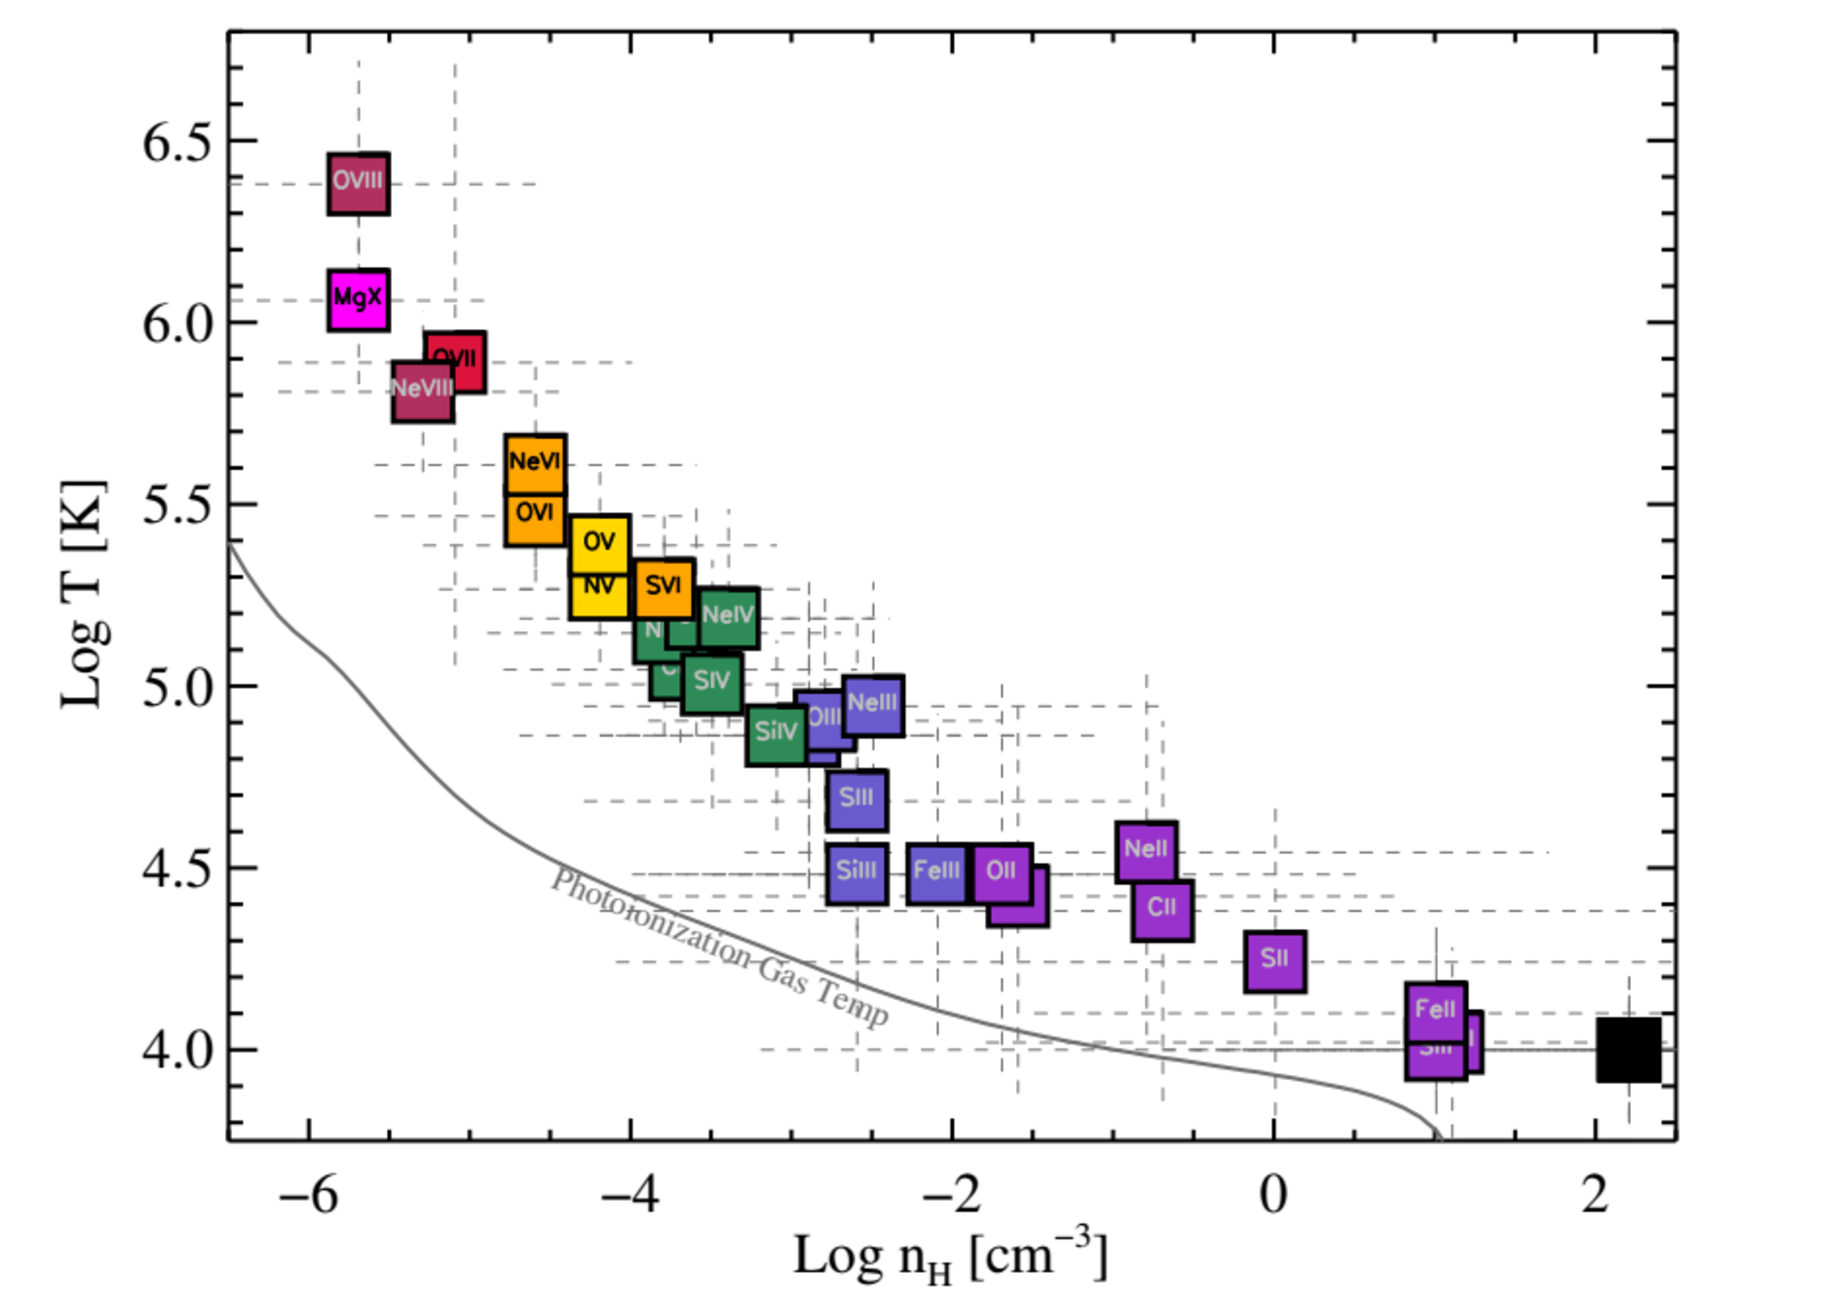
\includegraphics[angle=0]{Jess_plot}}}
%\caption[]{.}
%\label{}
%\end{figure}

%Related to the mysteries posed by the CGM, astronomers are also trying to understand how the quenching of galaxies, that is the ``turning off'' of star formation that leads to red elliptical galaxies, occurs. In particular, what causes galaxies to quench, and what sustains their lack of star formation? Some considerations of this dilemma include staunching IGM accretion which feeds the CG[cite, observations and sims!] and effects which keep the CGM hot enough that stars are unable to form, such stellar or AGN feedback or \textit{major?} mergers with other galaxies [Pontzen2017, cite more]. 

%Observationally, one common method of investigating the CGM is through line of sight observations of background QSOs. Studying the spectra of bright background objects allows us to examine the absorption features of the extended foreground gaseous media (including the CGM
%of galaxies nearby in projection) through which the QSO’s light filters [FIGURE?]. These absorption-line studies allow for the direct measurement of absorption features (characterizing the CGM) within the QSO spectra, allowing us to study the elusive CGM more directly. 

%\textbf{Intro 2: Discuss NBODY Sims} \\

%Cosmological hydrodynamic simulations are an important tool for understanding the underlying physics characterizing the CGM. Current smooth particle hydrodynamic (SPH) simulations utilize a dark-matter-only component and a follow-up zoom-in simulation to bridge the gap between large-scale galactic gravitational effect and the small-scale effects of gas, stars, and dust. Significant discoveries have already been made by investigating the CGM of simulated galaxies. Ford et al. (2013) determined that 65 -- 80 percent of the total baryon mass of a galaxy exists in the halo outside the stellar disk and that $\sim$80$\%$ of the fuel for star formation in the Milky Way Galaxy was in the CGM 1 billion years ago. However, most comparisons between simulation and data have primarily focused on bulk column density comparisons and largely ignored gas kinematics \citep {Stinson2012, Hummels2013, Ford2016a, Oppenheimer2016, Suresh2017}

%One of the most high resolution and recent cosmological simulation codes, ChaNGA, is a smoothed-particle hydrodynamics (SPH) code, which can directly examine the dynamics of the CGM in its simulated galaxies. Though comparable to the “Eris” simulations in mass and force resolution, ChaNGa has higher reliability when resolving high-density regions (Zolotov2012) and an improved implementation of black hole (BH) accretion, dynamics, and formation (Tremmel2016). These simulations allow us to determine kinematic information about the gas and metals residing in the CGM of these simulated galaxies and how it is affected by the BH and AGN activity. 

%\textbf{Intro 2: Discuss GM Sims} \\

%These “genetically modified” (GM) simulations of low redshift galaxies keep the large scale structure and cosmological conditions of $\alpha$ CDM consistent, while allowing for modifications of their accretion histories (Roth2015, more?). The analyses of these GM simulations allow for direct comparisons of the CGM of multiple versions of the same galaxy in a physically self-consistent treatment. Previous studies have  inspected the quenching mechanisms that arise from these varied accretion histories \citep{Pontzen2017}; however, they have not yet examined the dynamical effects on the CGM gas that these modified accretion histories generate.

%These genetically modified galaxies serve to further examine the questions posed by the CGM and its relation to quenching. We can look to the changes or similarities in the CGM amidst this suite of simulations to see how the subtle changes made to each of these Milky Way galaxies affect the CGM in a self-consistent way.

%The simulation parameters of the individual GM galaxies are described in Section 2. Simulation analysis methods are described in Section 3. Results are compiled in Section 4, and we summarize our findings in Section 5.


% ####### END OF INTRODUCTION #########
% #####################################


% #####################################
% ####### SIMULATION PARAMETERS #######
% #####################################

\section{Simulation Parameters}\label{sec-model}

% BELOW IS DM MASS TABLE; PROBABLY UNNECCESSARY
% \begin{table}[ht] % `*' makes it go across both columns instead of one
% \caption{Gas+BH Simulation Details} % title of Table
% \centering % used for centering table
% \begin{tabular}{c c c} % centered columns (4 columns)
% \hline\hline %inserts double horizontal lines
% Sim & Total Halo Mass & R$_{vir}$\\
%  & (M$_{\odot}$) & (kpc) \\ [0.5ex] % inserts table
% %heading
% \hline % inserts single horizontal line
% P0 & 9.91 $\times$ 10$^{11}$ & 262.3\\ % inserting body of the table
% GM1 & 1.02 $\times$ 10$^{12}$ & 264.5\\
% GM4 & 8.58 $\times$ 10$^{11}$ & 250.0\\
% GM5 & 9.08 $\times$ 10$^{11}$ & 254.7\\
% GM6 & 7.58 $\times$ 10$^{11}$ & 239.8\\ [1ex] % [1ex] adds vertical space
% \hline %inserts single line
% \end{tabular}
% \label{table:nonlin} % is used to refer this table in the text
% \end{table}

%Romulus & GMs: NO METAL LINE COOLING
%	Virial definitions + Galaxy masses: match Tully-Fischer, mass-metallicity, size-luminosity, SMHM
%	Star, gas, DM particle information
%	Star formation: requirements, histories, and IMF 
%	SN feedback
%	Cooling mechanisms
%	Metals: metal tracing? none
%	BH seeding and formation requirements, mergers: Michael!
%	Accretion model: Tremmel 2016
%	BH-bulge mass relation & luminosity function
%	BH feedback
%	Dynamical friction: Tremmel 2015

\subsection{ChaNGa Physics} 
Both ROMULUS25 (hereafter R25) and our set of zoom-in galaxies were run using the smoothed particle hydrodynamics (SPH) N-body tree code, Charm N-body GrAvity solver [ChaNGa]\citep{Menon2015}. ChaNGa includes the same models for a cosmic UV background, star formation, `blastwave' SN feedback, and low temperature metal line cooling as previously used in GASOLINE \citep{Wadsley2004,Wadsley2008,Stinson2006,Shen2010}. ChaNGa includes an improved SPH formalism which includes a geometric density approach in the force expression: (P$_i$ + P$_j$)/($\rho_i \rho_j$) instead of P$_i$/$\rho_{i}^2$ + P$_j$/$\rho_{j}^2$ where P$_i$ and $\rho_i$ are the particle's pressure and density, respectively. This update to the hydrodynamic treatment includes thermal diffusion \citep{Shen2010} and reduces artificial surface tension allowing for better resolution of fluid instabilities \citep{Ritchie2001,Menon2015,Governato2015}. Additional improvements have been made to the BH formation, accretion, and feedback models as well an improved prescription for dynamical friction \citep{Tremmel2015,Tremmel2017}. 

Our simulations were run with a $\Lambda$CDM cosmology from the most recent Planck collaboration utilizing $\sigma_0$ = 0.3086, $\alpha$ = 0.6914, h = 0.67, $\sigma_8$ = 0.77 and have Plummer equivalent force softening lengths of 250 pc. For simulating the cosmic reionization energy, both simulations enact a UV background at z $\sim$ 9 \citep{Haardt2012}.

\subsection{Romulus 25 Cosmological Volume}
The ROMULUS25 \citep{Tremmel2017} simulation is a cosmological volume which includes galaxy halos within the mass range 10$^{8}$ \textemdash 10$^{13}$ M$_{\odot}$. R25 has a mass resolution of 3.4 $\times$ 10$^5$ M$_{\odot}$ and 2.1 $\times$ $10^5$ M$_{\odot}$ for DM and gas particles, respectively. For our study, we focus on galaxies within the MW-mass halo regime, 5 $\times$ 10$^{11}$ M$_{\odot}$ \textemdash  2 $\times$ 10$^{12}$ M$_{\odot}$ (Figure \ref{ROMhist}). We examine all the galaxies within the specified mass range and exclude any galaxies within twice the virial radius of another galaxy, thereby removing galaxies that might be satellites of a larger galaxy. With these selection criteria in place, our sample includes 25 galaxies.

\begin{figure}[]
\centerline{\resizebox{1.02\hsize}{!}{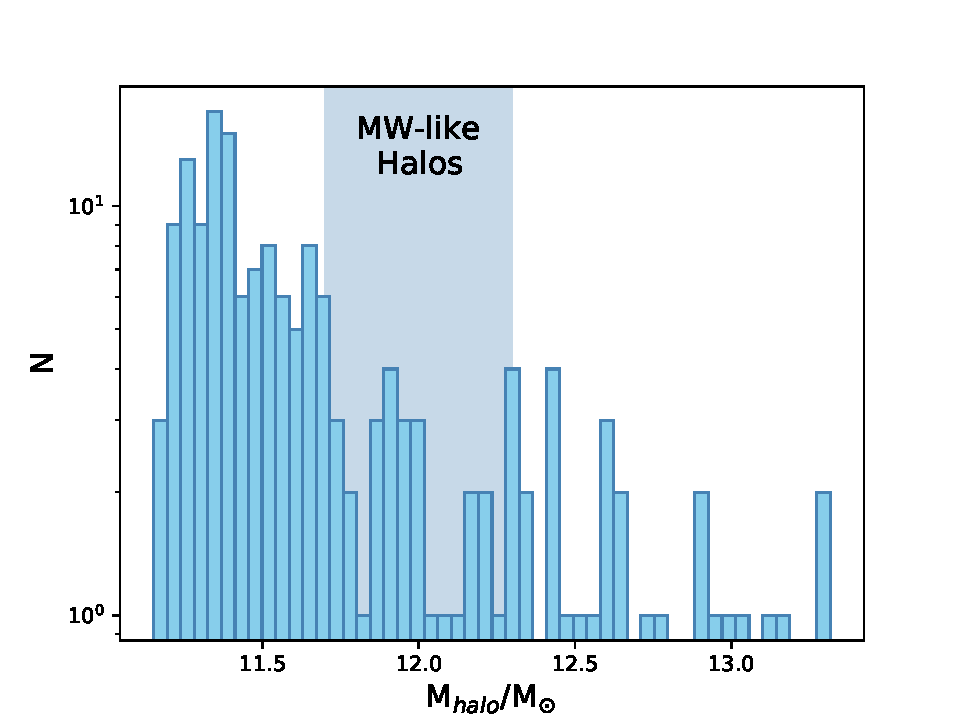
\includegraphics[angle=0]{ROMhistogram}}}
\caption[]{R25 is an SPH simulated cosmological volume with galaxy halos spanning the orders of 10$^{8}$ \textemdash 10$^{13}$ M$_{\odot}$. For clarity, we've plotted a histogram of only the galaxies in the volume with masses between 2 $\times$ 10$^{11}$ M$_{\odot}$ \textemdash 2 $\times$ 10$^{13}$ M$_{\odot}$ (The latter is the upper limit of galaxy masses in the volume.) The shaded region indicates the ``MW'' mass range, 5 $\times$ 10$^{11}$ M$_{\odot}$ \textemdash  2 $\times$ 10$^{12}$ M$_{\odot}$, from which we select our 25 galaxies.}
\label{ROMhist}
\end{figure}

\subsection{Zoom-In Galaxies: Patient 0 and its Genetic Modifications}
To select our galaxy, we ran initial uniform-volume, 50 h$^{-1}$ Mpc on a side, dark matter-only cosmological volume. From this volume a MW-mass halo at z=0, was selected as our ``Patient 0'' and then re-simulated at a higher resolution. For the subsequent, ``genetically modified'' (GM) zoom-in runs, we utilize the same method of modification as \cite{Pontzen2016}. These GM simulations keep the large scale structure and cosmological conditions $\Lambda$CDM consistent (as in Patient 0), while allowing for modifications of their accretion histories (Roth et al., 2015). Patient 0 (and its 3 GM simulations) have a mass resolutions of 1.4 $\times$ 10$^5$ M$_{\odot}$ and 2.1 $\times$ $10^5$ M$_{\odot}$ for DM and gas particles, respectively. The DM field in these galaxies is simulated at twice the gas linear resolution to reduce noise in the potential near the galactic center \citep{Pontzen2016} and more accurately trace black hole dynamics \citep{Tremmel2015}.

\subsubsection{Galaxies with BH Physics} 

\begin{table*}[ht!] % `*' makes it go across both columns instead of one
\caption{Zoom-In Galaxies Properties \textit{with BHs} at z = 0.17 \textit{Values that have been updated are italicized}} % title of Table
\centering % used for centering table
\begin{tabular}{c c c c c c c c} % centered columns (4 columns)
\hline\hline %inserts double horizontal lines
Sim & Total Halo Mass  & Total Gas Mass & Total Stellar Mass & CGM Gas Mass & R$_{vir}$ & T$_{vir}$ & \textbf{Satellite Mass}\\
 & (M$_{\odot}$) & (M$_{\odot}$) & (M$_{\odot}$) & (M$_{\odot}$) & (kpc) & (K) & \textbf{(M$_{\odot}$)} \\ [0.5ex] % inserts table
%heading
\hline % inserts single horizontal line 
P0 & 1.08 $\times$ 10$^{12}$ & 1.09 $\times$ 10$^{11}$ & 5.71 $\times$ 10$^{10}$ & \textit{9.32 $\times$ 10$^{10}$} & 268.9 & 5.12 $\times$ 10$^5$ & \textbf{7.34 $\times$ 10$^{10}$}\\ % inserting body of the table
GM1 & 1.07 $\times$ 10$^{12}$ & 1.01 $\times$ 10$^{11}$ & 6.43 $\times$ 10$^{10}$ & \textit{8.39 $\times$ 10$^{10}$} & 269.2 & 5.12 $\times$ 10$^5$ & \textbf{5.86 $\times$ 10$^{10}$}\\
GM2 & 8.69 $\times$ 10$^{11}$ & 7.41 $\times$ 10$^{10}$ & 1.38 $\times$ 10$^{10}$ & \textit{6.89 $\times$ 10$^{10}$} & 254.1 & X $\times$ 10$^5$ & \textbf{3.97 $\times$ 10$^{10}$}  \\ % This used to be GM7
GM3 & 7.76 $\times$ 10$^{11}$ & 6.36 $\times$ 10$^{10}$ & 1.04 $\times$ 10$^{10}$ & \textit{5.02 $\times$ 10$^{10}$} & 241.7 & 4.14 $\times$ 10$^5$ & \textbf{2.45 $\times$ 10$^{10}$} \\ [1ex] % [1ex] adds vertical space; GM3 used to be GM4
\hline %inserts single line
\end{tabular}
\label{table:BHdata} % is used to refer this table in the text


\end{table*}\begin{table*}[ht] % `*' makes it go across both columns instead of one
\caption{Zoom-In Galaxies Properties \textit{without BHs} at  z = 0.17} % title of Table
\centering % used for centering table
\begin{tabular}{c c c c c c c c} % centered columns (4 columns)
\hline\hline %inserts double horizontal lines
Sim & Total Halo Mass  & Total Gas Mass & Total Stellar Mass & CGM Gas Mass & R$_{vir}$ & T$_{vir}$ & \textbf{Satellite Mass}\\
 & (M$_{\odot}$) & (M$_{\odot}$) & (M$_{\odot}$) & (M$_{\odot}$) & (kpc) & (K) & \textbf{(M$_{\odot}$)} \\ [0.5ex] % inserts table
%heading
\hline % inserts single horizontal line
P0noBH & 8.36 $\times$ 10$^{11}$ & 7.0 $\times$ 10$^{10}$ & 7.37 $\times$ 10$^{10}$ & X $\times$ 10$^{10}$ & 262.8 & X $\times$ 10$^5$ & \textbf{7.34 $\times$ 10$^{10}$}\\ % inserting body of the table
GM1noBH & 8.38 $\times$ 10$^{11}$ & 7.07 $\times$ 10$^{10}$ & 7.34 $\times$ 10$^{10}$ & X $\times$ 10$^{10}$ & 263.0 & X $\times$ 10$^5$ & \textbf{5.86 $\times$ 10$^{10}$}\\
GM2noBH & 8.42 $\times$ 10$^{11}$ & 7.08 $\times$ 10$^{10}$ & 7.33 $\times$ 10$^{10}$ & X $\times$ 10$^{10}$ & 263.4 & X $\times$ 10$^5$ & \textbf{3.97 $\times$ 10$^{10}$}  \\ % This used to be GM7
GM3noBH & 8.43 $\times$ 10$^{11}$ & 7.19 $\times$ 10$^{10}$ & 7.28 $\times$ 10$^{10}$ & X $\times$ 10$^{10}$ & 263.5 & X $\times$ 10$^5$ & \textbf{2.45 $\times$ 10$^{10}$} \\ [1ex] % [1ex] adds vertical space; GM3 used to be GM4
\hline %inserts single line
\vspace{5.111mm}
\end{tabular}
\label{table:noBHdata} % is used to refer this table in the text
\end{table*}



At z = 0, our ``Patient 0'' (hereafter P0) galaxy is a star forming galaxy with a disk (Figure \ref{sfh}a). P0 has an incoming satellite at z = 1 with an original mass of 7.34 $\times$ 10$^{10}$ M$_{\odot}$ (mass ratio, q = 0.12). For each GM galaxy simulation, we systematically shrink this satellite halo's mass prior to its merger with the main halo. (Table \ref{table:BHdata}) GM1 results in a similar disked, star forming galaxy as P0, while GM2 and GM3 become quenched at z $\sim$ 1 (Figure \ref{sfh}a). 

%\textit{GM1:} For our first GM galaxy, we shrink the satellite halo's mass to 5.86 $\times$ 10$^{10}$ M$_{\odot}$ (q = 0.10). At z = 0, GM1 is a star forming galaxy (Figure \ref{sfh}a) with a disk and has a final halo mass of 1.07 $\times$ 10$^{12}$ and R$_{vir}$ = 269 kpc. It has total gas and stellar masses of 1.01 $\times$ 10$^{11}$ M$_{\odot}$ and 6.43 $\times$ 10$^{10}$ M$_{\odot}$, respectively.

%\textit{GM2:} Our second GM galaxy has a incoming satellite mass shrunk to 3.97 $\times$ 10$^{10}$ M$_{\odot}$ (q = 0.06). At z = 0, GM2 has a final halo mass of 8.69 $\times$ 10$^{11}$ M$_{\odot}$ and R$_{vir}$ = 254 kpc. It has total gas and stellar masses of 7.41 $\times$ 10$^{10}$ M$_{\odot}$ and 1.38 $\times$ 10$^{10}$ M$_{\odot}$, respectively.

%\textit{GM3:} The third and final GM galaxy has a incoming satellite mass shrunk to 2.45 $\times$ 10$^{10}$ M$_{\odot}$ (q = 0.04). At z = 0, GM3 has a final halo mass of 7.76 $\times$ 10$^{11}$ M$_{\odot}$ and R$_{vir}$ = 242 kpc. It has a total gas and stellar masses of 6.36 $\times$ 10$^{10}$ M$_{\odot}$ and 1.04 $\times$ 10$^{10}$ M$_{\odot}$, respectively. 

While the GM galaxies utilize the same process as \cite{Pontzen2016}, their study examines a different set of galaxies. The three galaxies in \cite{Pontzen2016} were run to z = 2 and have M$_{Halo}$ $\sim$ 10$^{12}$. They each have incoming satellites whose masses are both increased and decreased prior to merging with the main galaxy, as in our galaxies; however, the resulting effect of their modifications were different from ours, as we explore in Section \ref{Discuss}.

\subsubsection{Galaxies without BH Physics}
One key benefit of the individual zoom-in galaxies include the ability to remove or adjust the physical parameters affecting our galaxies to test different theoretical models which would be too computationally expensive to do with a large volume like R25. We utilize this benefit to further understand the effects of the AGN. To isolate the effect of the AGN on the CGM, all four of the zoom-in simulations (P0 and its 3 GMs) were re-simulated at the same resolution and with all the same physics \textit{excluding} BH formation, feedback, and dynamical friction (Table \ref{table:noBHdata}). Black hole seed formation was disabled and the BH feedback and accretion efficiency parameters were set to 0.

\begin{figure}[h!]
\centerline{\resizebox{0.98\hsize}{!}{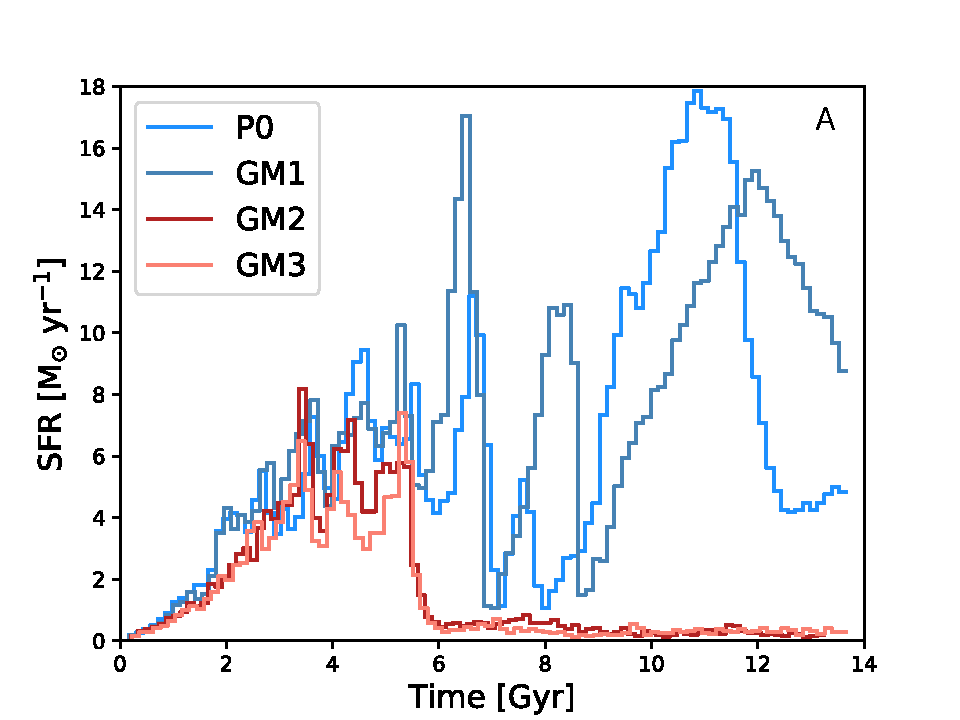
\includegraphics[angle=0]{ALLBH_sfh}}}
\vspace{-1mm}
\centerline{\resizebox{0.98\hsize}{!}{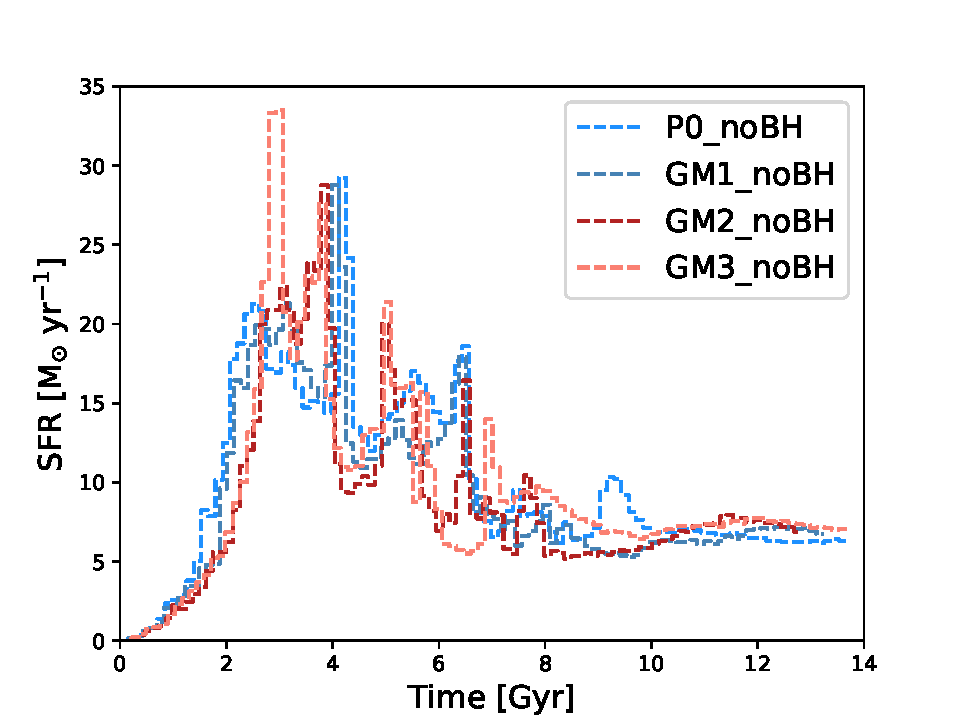
\includegraphics[angle=0]{ALLnoBH_sfh}}}
\caption[]{The star formation histories for the zoom-in galaxies: Patient 0 and its 3 GM galaxies with BH physics (\textit{Upper}) and \textit{Lower} without BH physics. In the galaxies including BH physics, P0 and GM1 remain star forming throughout their histories while GM2 and GM3 become quenched at z $\sim$ 1. Without BH physics, all four galaxies remain star forming until z = 0. This is an effect we will explore in future work.}
\label{sfh}
\end{figure}

\begin{figure}[h!]
%\centerline{\resizebox{0.98\hsize}{!}{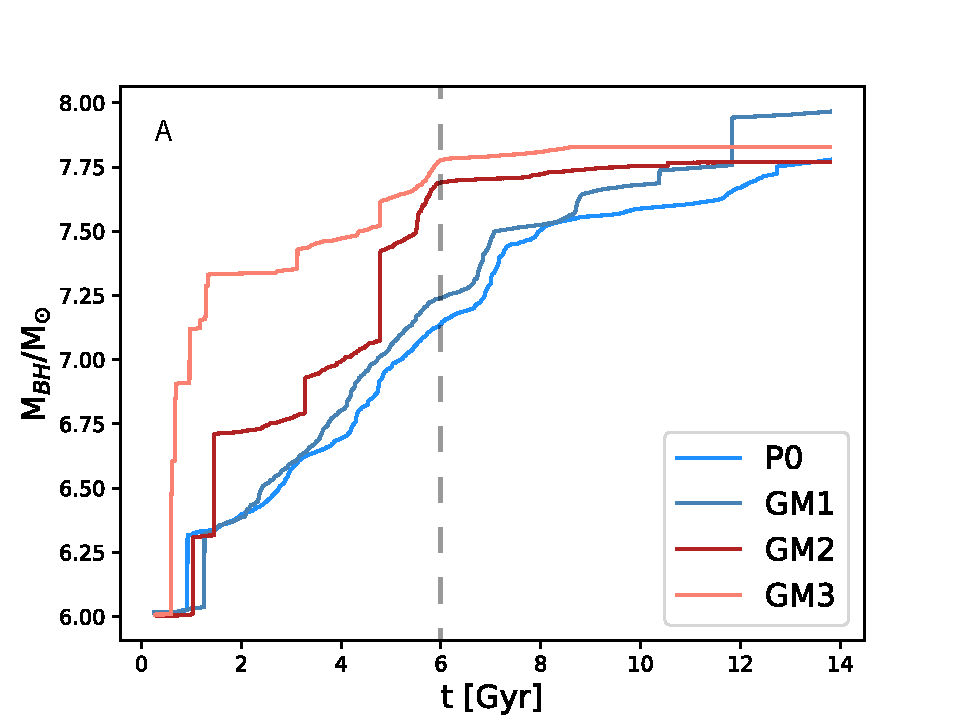
\includegraphics[angle=0]{ALLGM_BHmass}}}
%\centerline{\resizebox{0.98\hsize}{!}{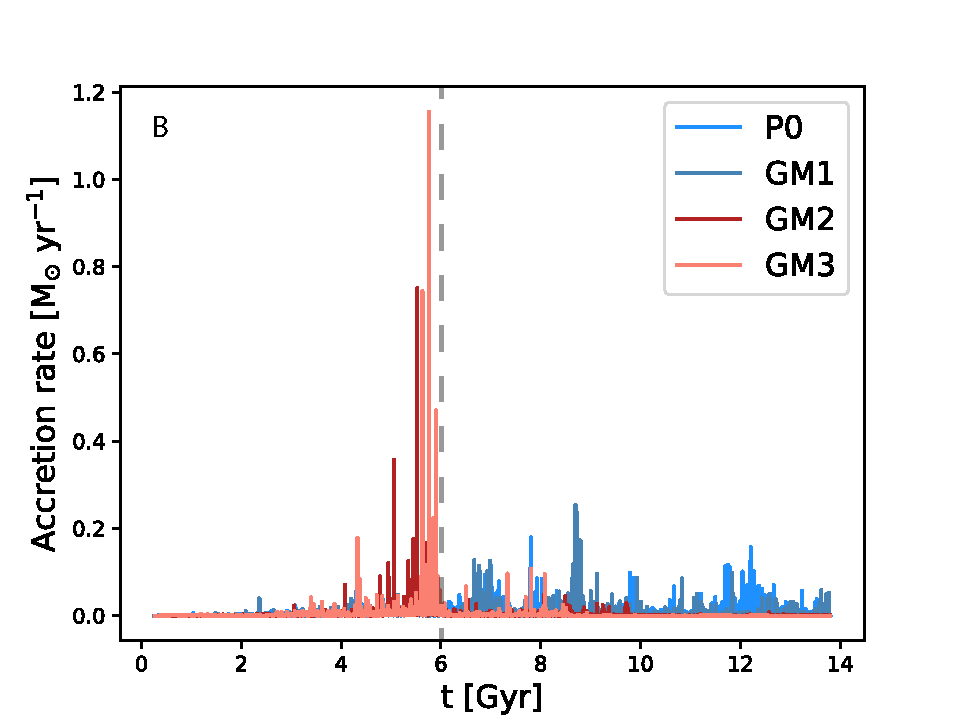
\includegraphics[angle=0]{ALLGM_BHaccrrate}}} 
\centerline{\resizebox{0.98\hsize}{!}{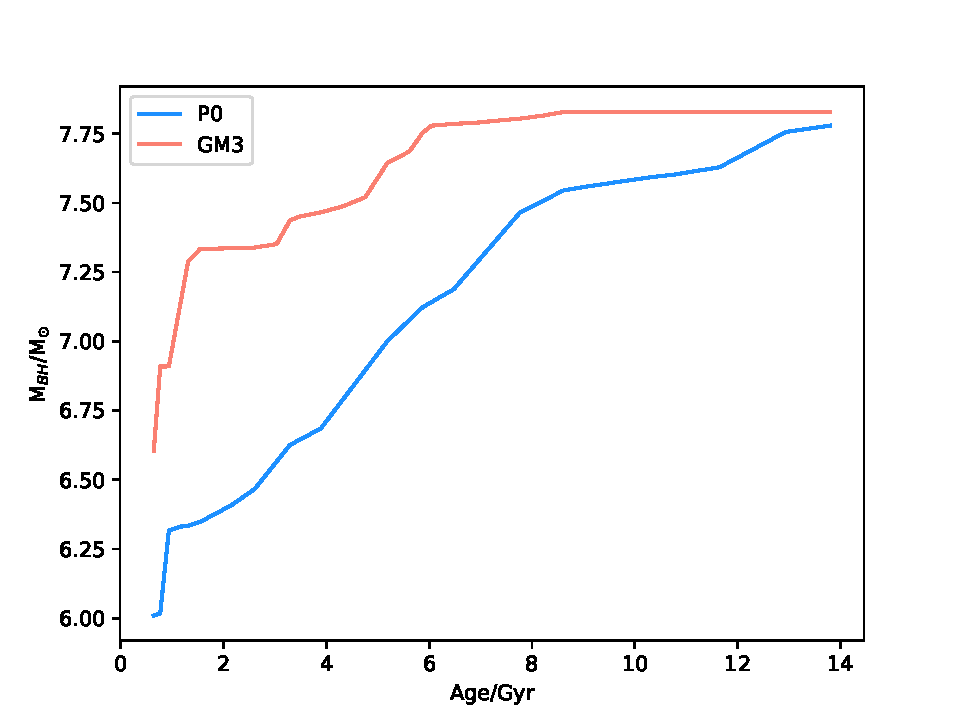
\includegraphics[angle=0]{P0_GM4_bhmass_age}}}
\centerline{\resizebox{0.98\hsize}{!}{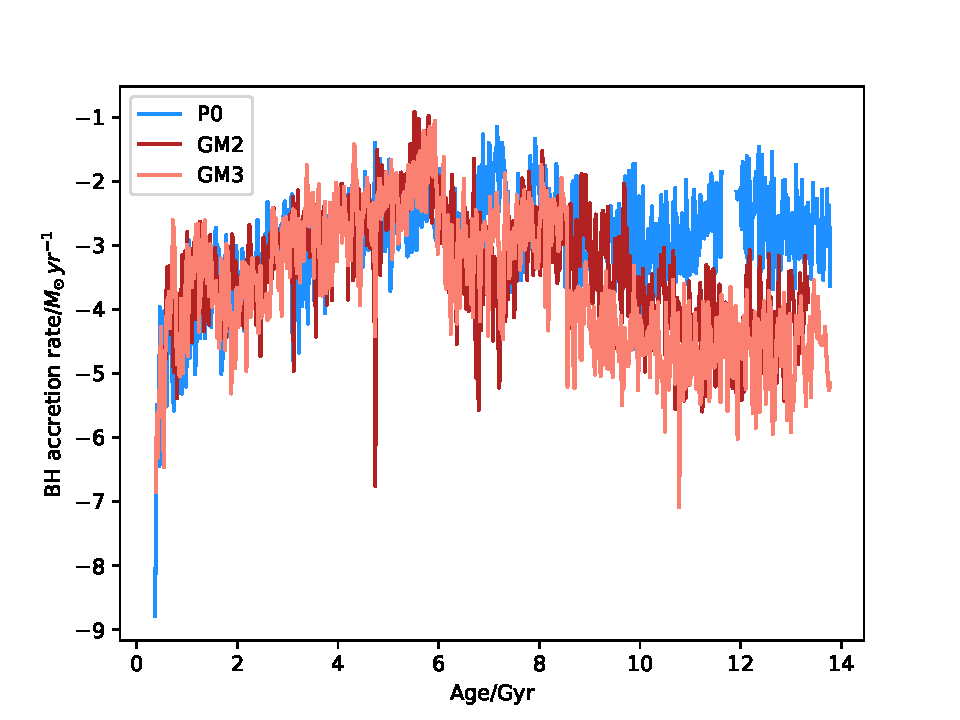
\includegraphics[angle=0]{P0_GM4and7_bhaccr_age}}} 
\caption[]{SMBH mass (\textit{Upper}) and SMBH accretion rates (\textit{Lower}) for our 4 zoom-in galaxies. Colors as in Figure \ref{GMandNOBH_Novi_vs_b}. The SMBH growth of GM2 and GM3 occurs quicker than the growth of the SMBH in the two star forming zoom-in galaxies. In particular, GM3, which has the most significant modification to its satellite's mass, has a SMBH that grows quickest. Both quenched galaxies also have a sharp peak in accretion rate around the time of the merger with the satellite (z $\sim$ 1, t $\sim$ 6 Gyr), indicated by the dashed grey line.}
\label{BHinfo}
\end{figure}

\subsubsection{Quenching in GM2 and GM3}
Particularly of note, the top panel of Figure \ref{sfh}, which shows star formation histories of the four zoom-in galaxies with BH physics included, clearly shows that unlike P0 and GM1 which remain star forming throughout their history, GM2 and GM3 become quenched at z $\sim$ 1. This immediate quenching just after the merger of the satellite with the main halo is particularly interesting because it does not take effect in the set of zoom-in galaxies without BH physics. Contrastingly, the lower panel of Figure \ref{sfh} shows the star formation histories of the four zoom-in galaxies without BH physics and all four of their histories are nearly identical. The stark differences between the GM2 and GM3 galaxies with and without BHs imply that some interplay between the satellite's mass and the AGN feedback must play a pivotal role in quenching these galaxies so thoroughly. 

We further examine the effects of the BH by looking to the mass buildup and accretion rate of the BHs. The upper panel in Figure \ref{BHinfo} shows the SMBH mass as a function of time. Here we see that the mass growth in the quenched galaxies, GM2 and GM3, occurs earlier in comparison to the star forming galaxies, especially in the case of GM3. A similar result can also be seen in lower panel of Figure \ref{BHinfo} which depicts the SMBH accretion rate as a function of time. It is clear from this figure that an increase of accretion occurs near the time of the merger, z $\sim$ 1 or t $\sim$ 6 Gyr. It is clear from the BH's activity and growth that the effect of the mass of the incoming satellite has profound affect on the assembly history of this galaxy. \cite{Pontzen2016} previously explored the relationship between BH feedback and mergers and its effect on quenching, using the same genetic modification technique as we use for the GM galaxies in our study. They determine that AGN feedback is critical to quenching a galaxy, which is consistent with our finding that the only quenched galaxies are in simulations that include SMBHs. \cite{Pontzen2016} argues that the merger can disrupt the cold disk of the galaxy, which then allows the feedback of the AGN to have a farther reaching effect on the star forming gas of the disk thereby keeping the galaxy in a state of quiescence. We note however, that the genetic modifications performed on the galaxies of \citep{Pontzen2016} was different from the ones implemented here. In their case, it was an increase of the satellite's mass that resulted in a quenched galaxy, rather than a shrinking as we affect here.

This set of galaxies, which were produced from very similar initial conditions but which illustrate very different star formation and accretion histories, allows us to directly examine how assembly history may imprint itself on the CGM. However, the specific effects of the AGN's accretion on the assembly history of the galaxy is beyond the scope of this paper. We leave an examination of the quenching mechanisms of these galaxies to future work. 

% ### END OF SIMULATION PARAMETERS ####
% #####################################


% #####################################
% ############# RESULTS ###############
% #####################################

\section{Results}\label{redux}

\begin{figure*}[h!]
\centerline{\resizebox{0.45\hsize}{!}{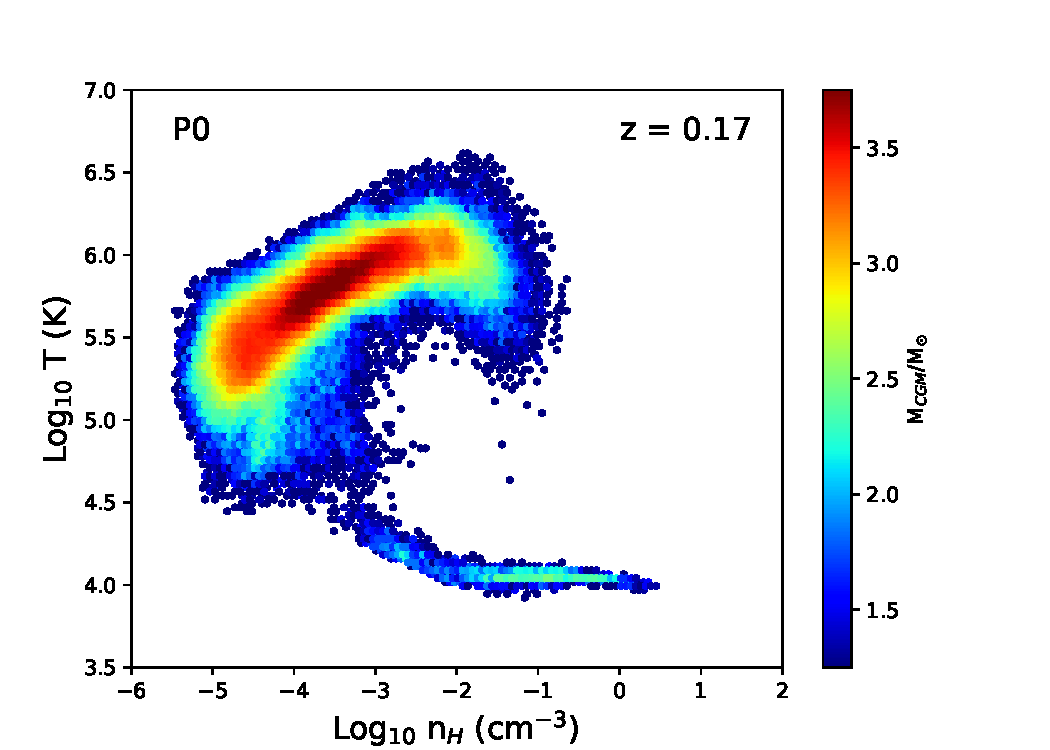
\includegraphics[angle=0]{P0_phasediagram_mass}}
\resizebox{0.45\hsize}{!}{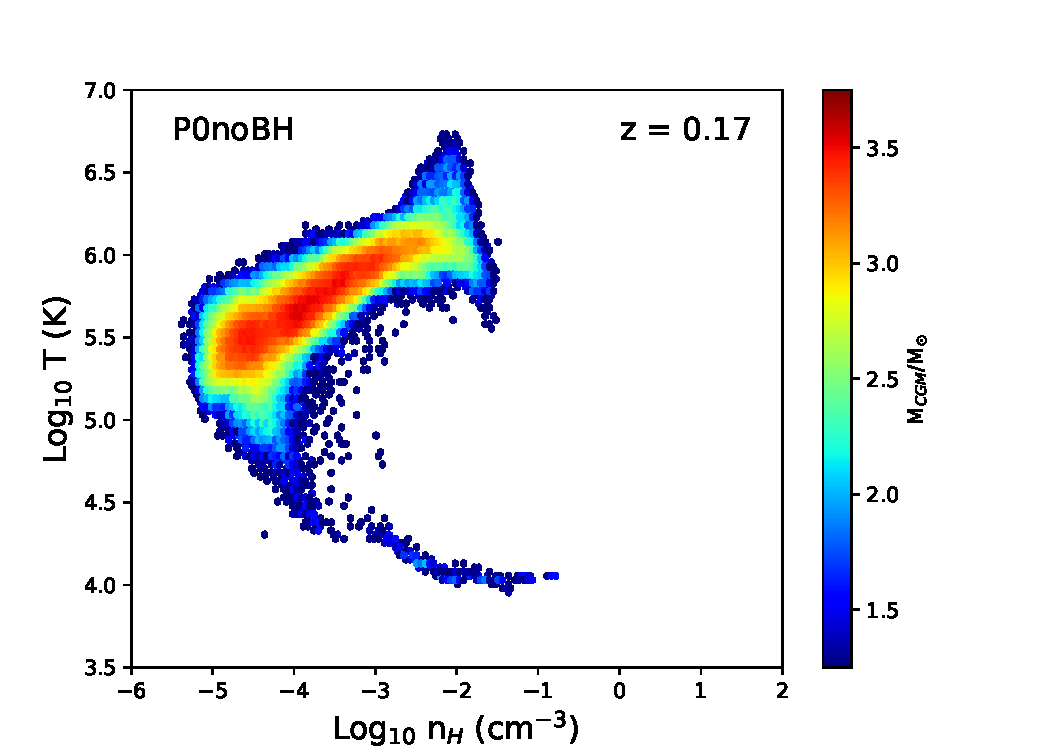
\includegraphics[angle=0]{P0noBH_phasediagram_mass}}}

\centerline{\resizebox{0.45\hsize}{!}{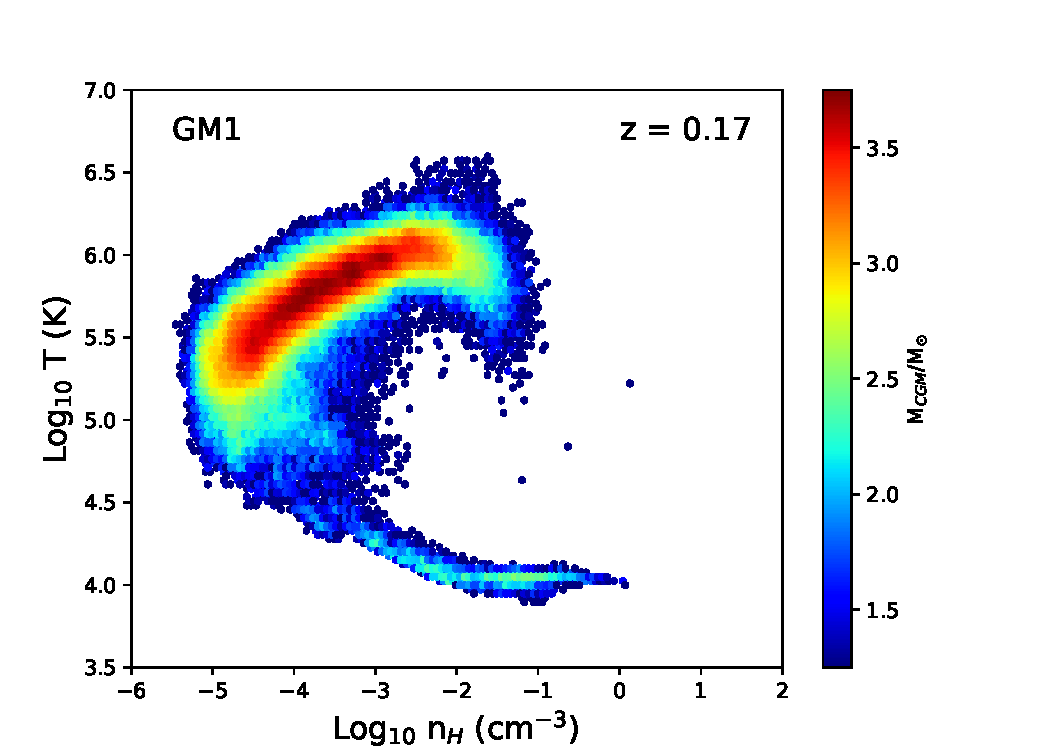
\includegraphics[angle=0]{GM1_phasediagram_mass}}
\resizebox{0.45\hsize}{!}{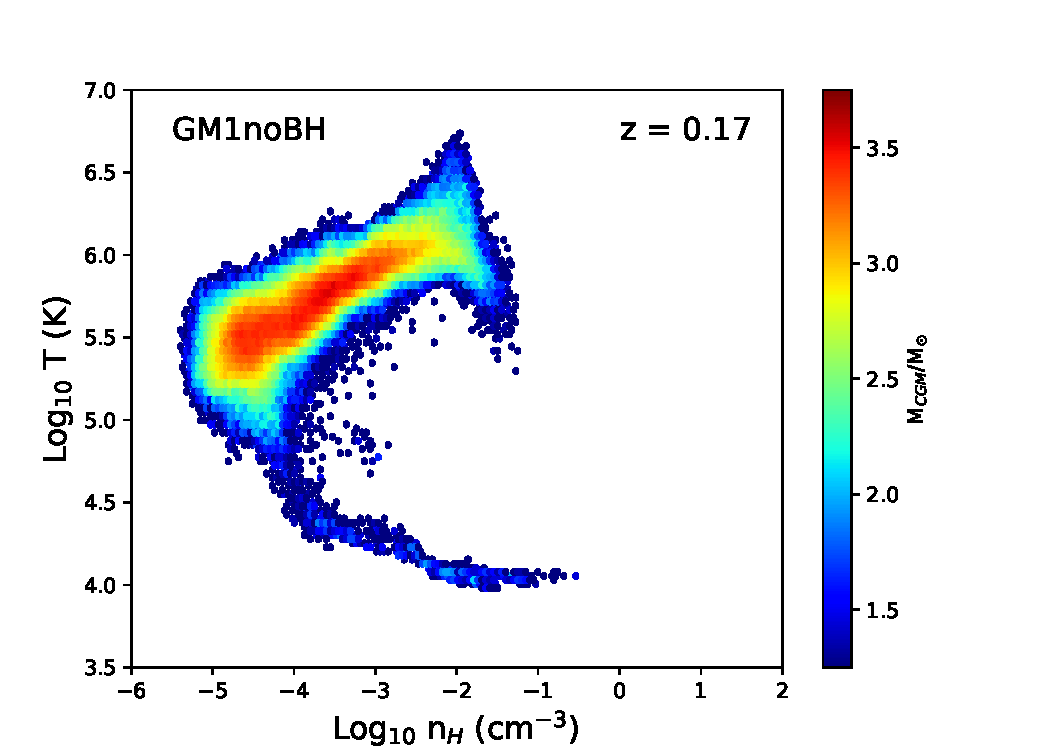
\includegraphics[angle=0]{GM1noBH_phasediagram_mass}}}

\centerline{\resizebox{0.45\hsize}{!}{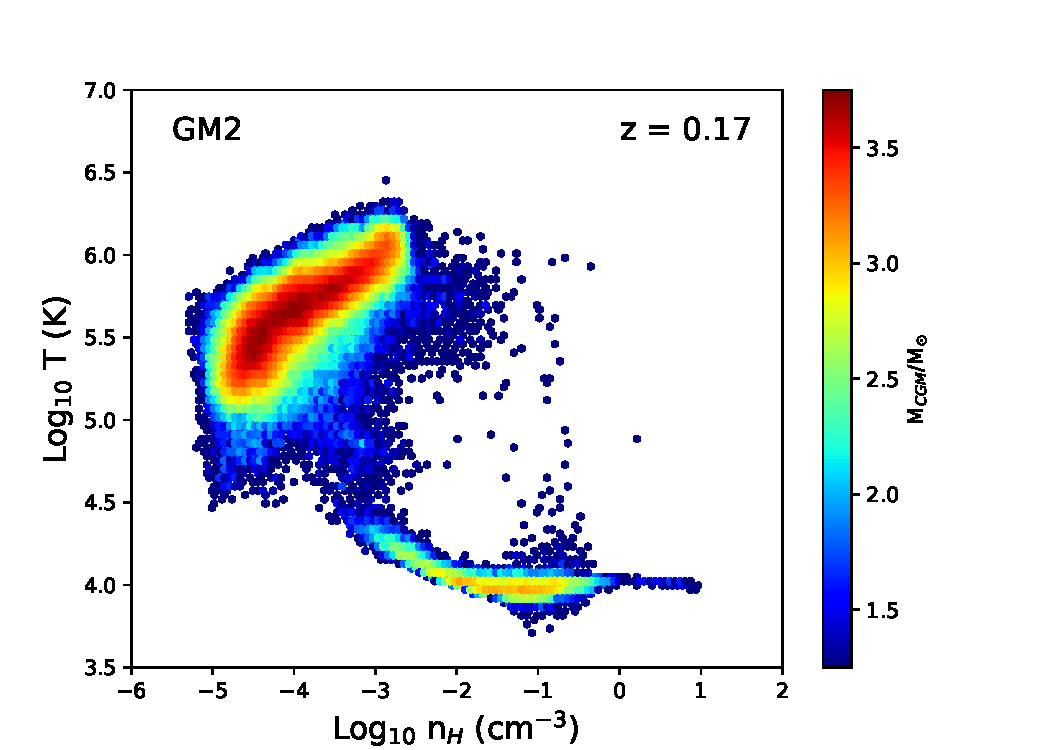
\includegraphics[angle=0]{GM2_phasediagram_mass}}
\resizebox{0.45\hsize}{!}{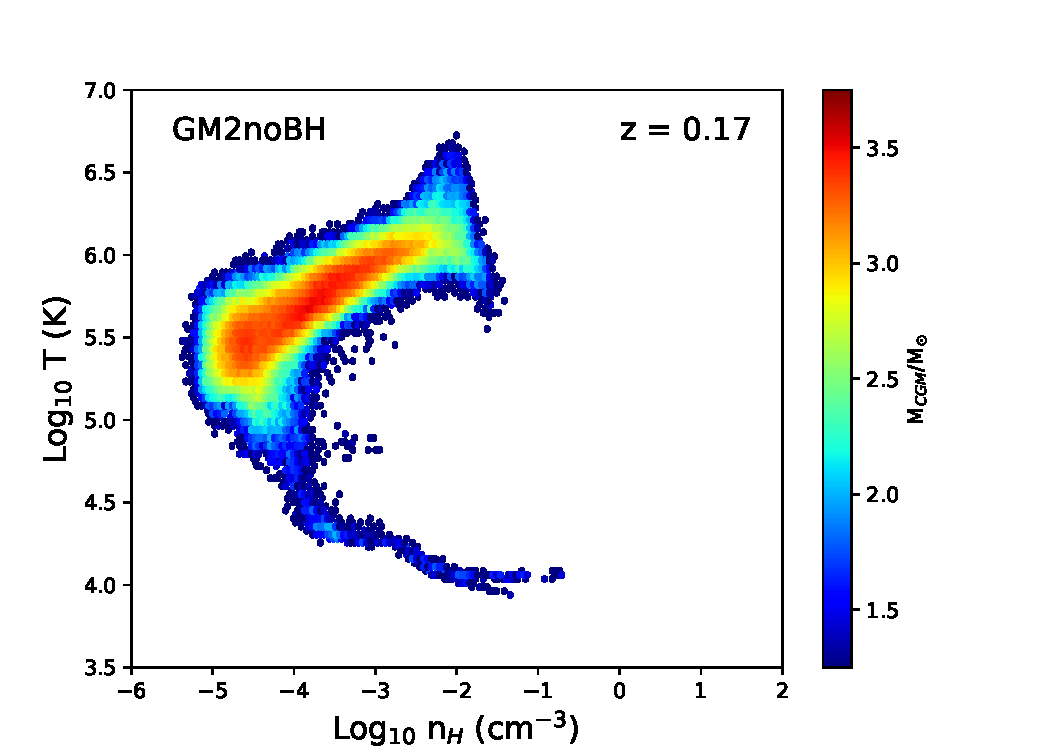
\includegraphics[angle=0]{GM2noBH_phasediagram_mass}}}

\centerline{\resizebox{0.45\hsize}{!}{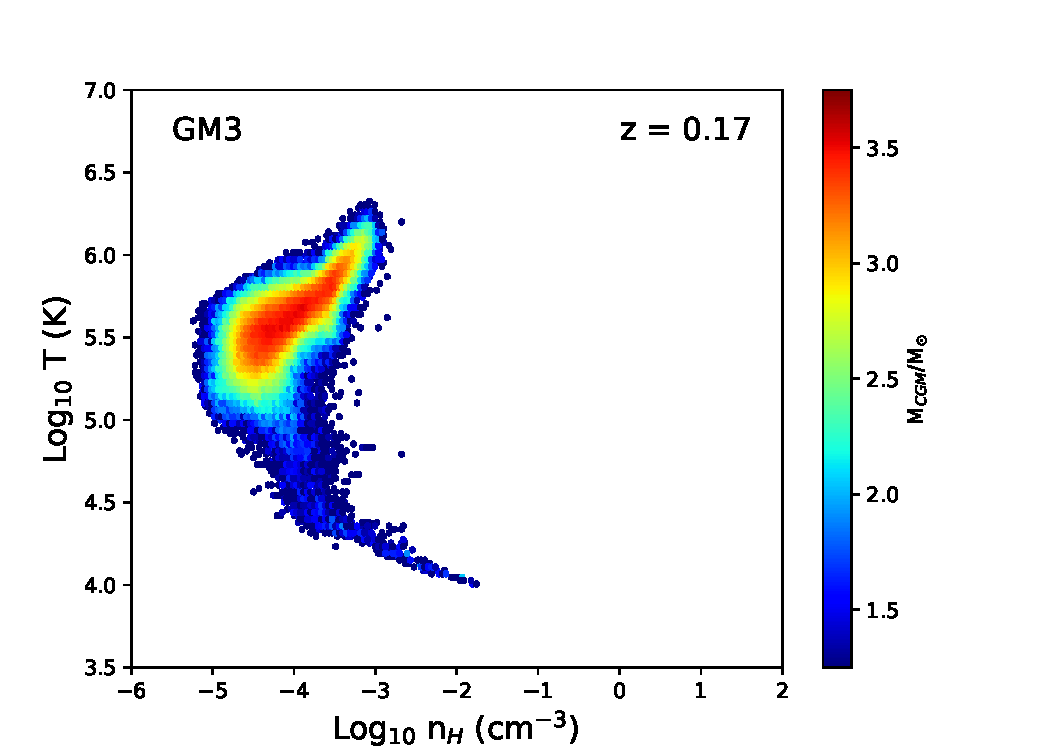
\includegraphics[angle=0]{GM3_phasediagram_mass}}
\resizebox{0.45\hsize}{!}{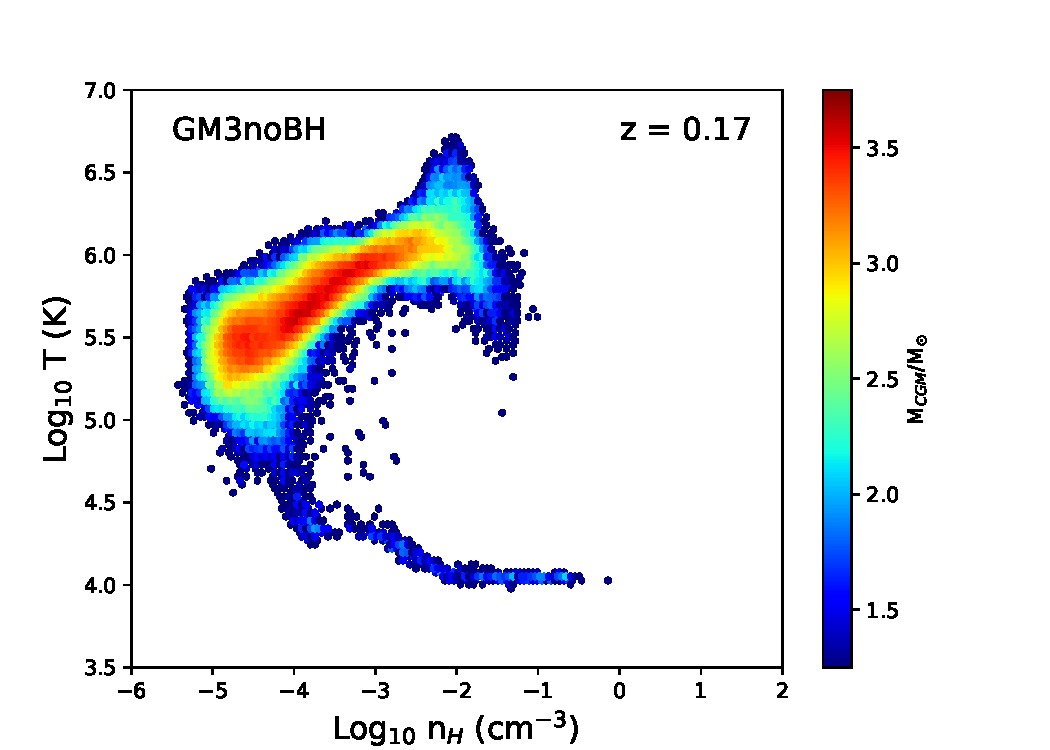
\includegraphics[angle=0]{GM3noBH_phasediagram_mass}}}
\caption[]{Phase diagrams of the temperature and density of the two star forming zoom-in galaxies, P0 (\textit{Top row}) and GM1 (\textit{Second row}), and the two quenched galaxies, GM2 (\textit{Third row}) and GM3 (\textit{Bottom row}). The phase diagrams of galaxies with BH hole physics vary quite widely between the star forming (P0 and GM1) and quenched cases (GM2 and GM3), particularly in the highest temperature and density gas. However, the phase diagrams of the galaxies without BH physics appear nearly identical, as do their star formation histories (Figure \ref{sfh} lower panel).}
\label{phasediagrams}
\end{figure*}


\begin{figure*}[h!]
\centerline{\resizebox{0.35\hsize}{!}{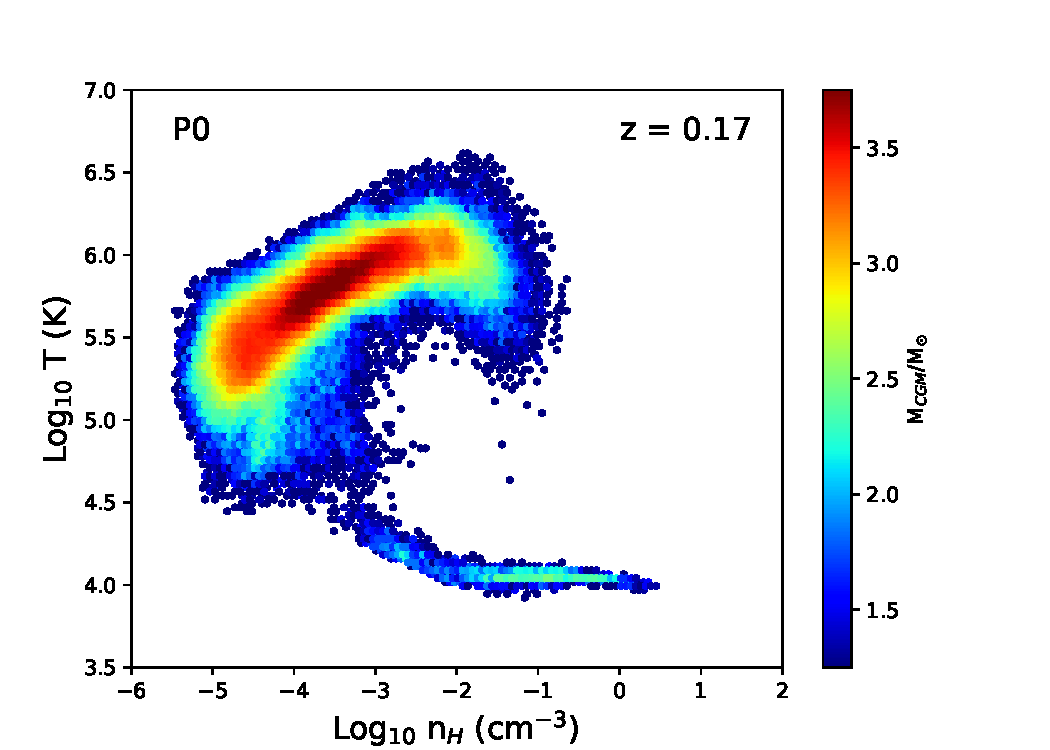
\includegraphics[angle=0]{P0_phasediagram_mass}}
\resizebox{0.35\hsize}{!}{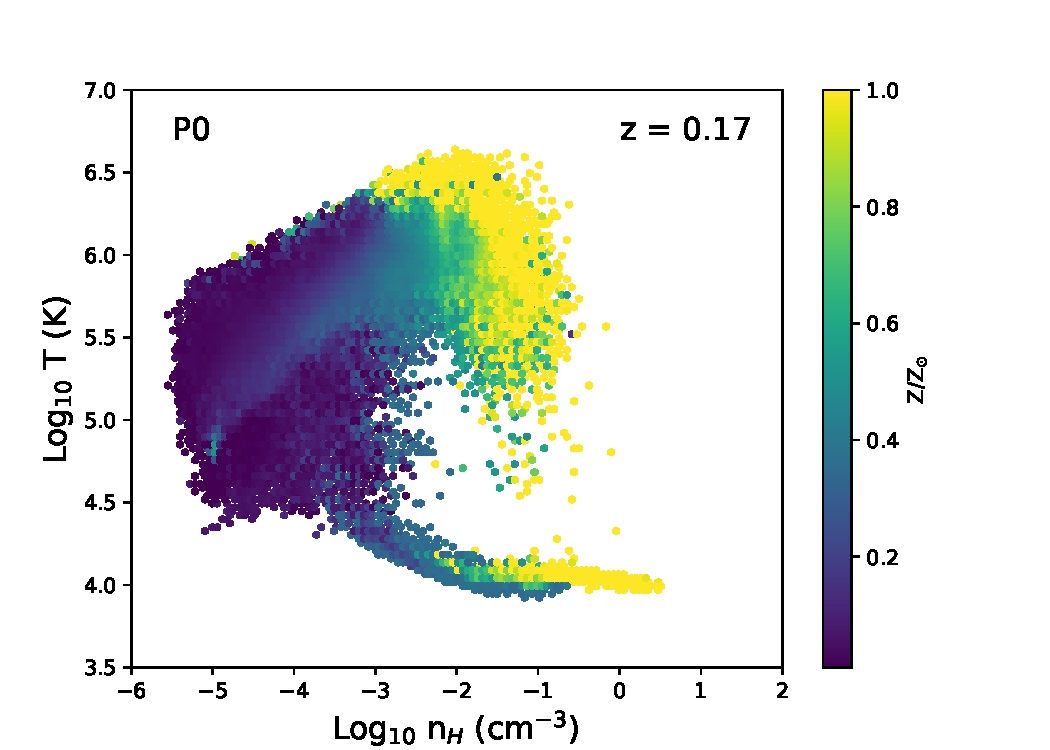
\includegraphics[angle=0]{P0_phasediagram_metallicity}}
\resizebox{0.35\hsize}{!}{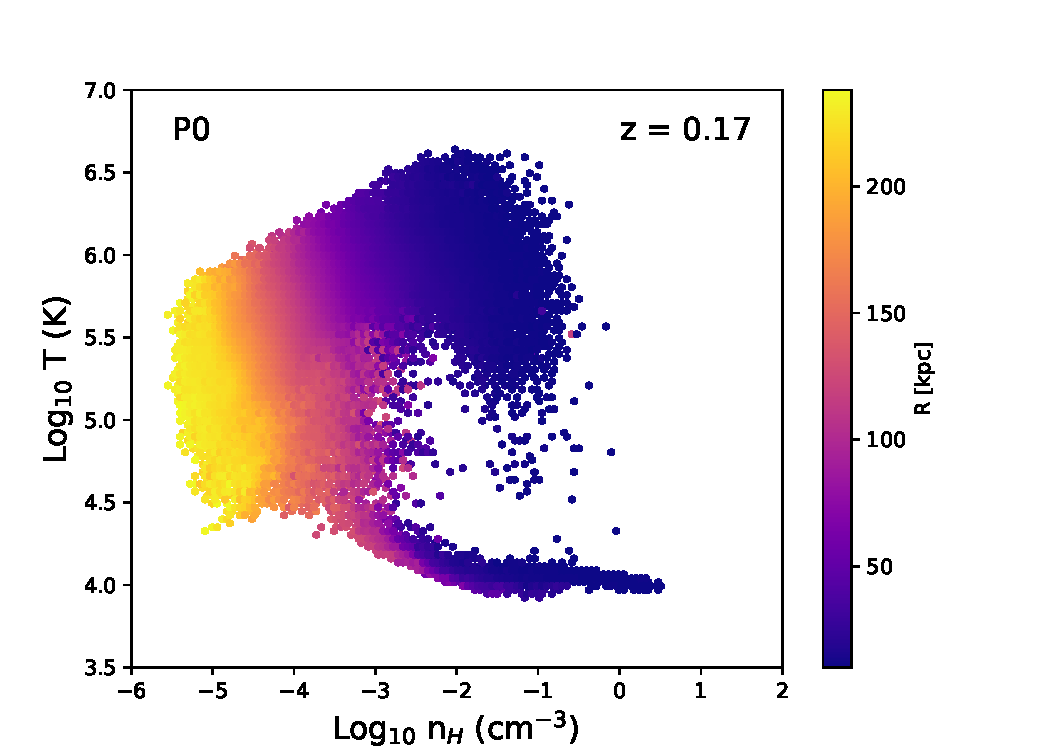
\includegraphics[angle=0]{P0_phasediagram_Rkpc}}}

\centerline{\resizebox{0.35\hsize}{!}{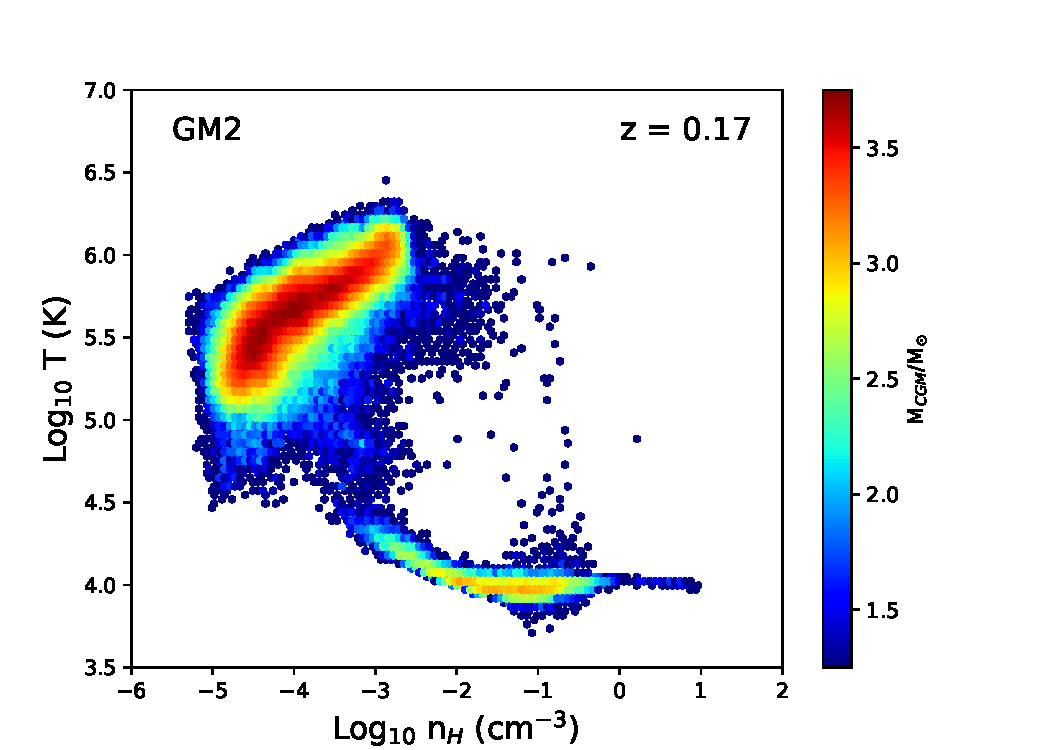
\includegraphics[angle=0]{GM2_phasediagram_mass}}
\resizebox{0.35\hsize}{!}{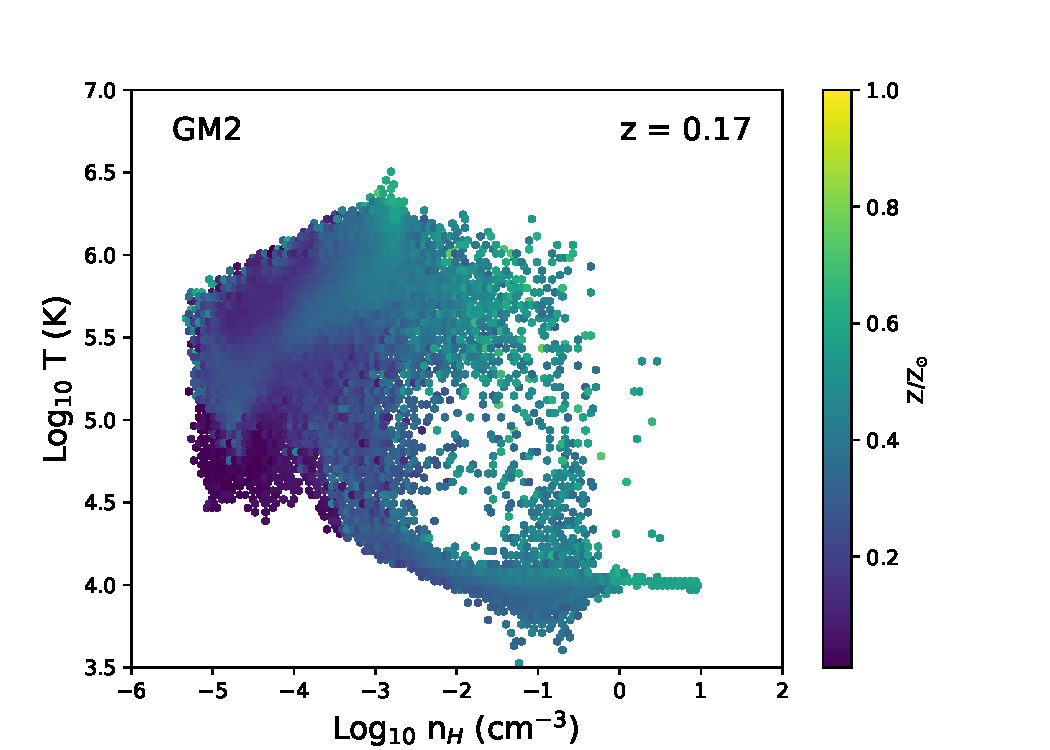
\includegraphics[angle=0]{GM2_phasediagram_metallicity}}
\resizebox{0.35\hsize}{!}{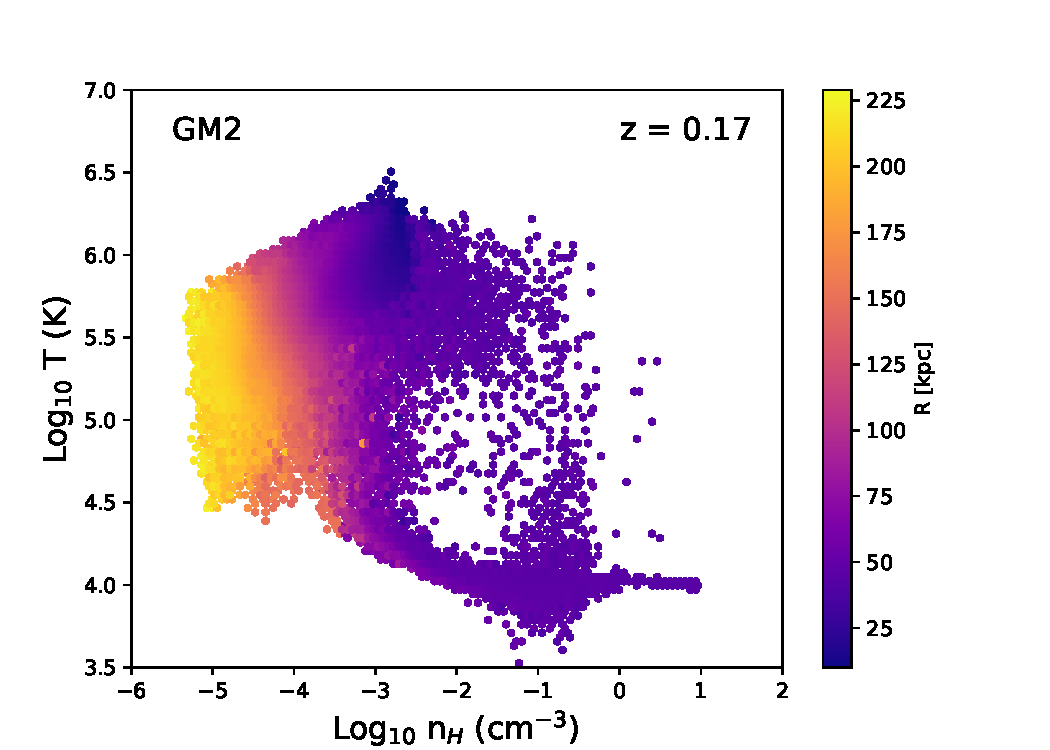
\includegraphics[angle=0]{GM2_phasediagram_Rkpc}}}

\centerline{\resizebox{0.35\hsize}{!}{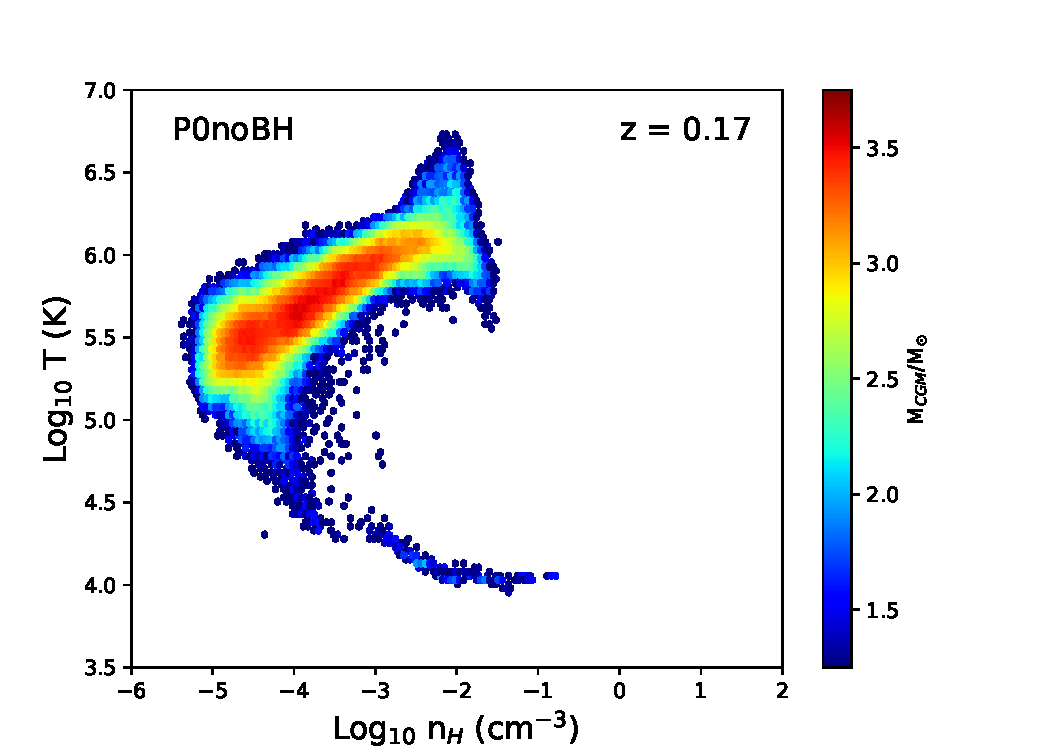
\includegraphics[angle=0]{P0noBH_phasediagram_mass}}
\resizebox{0.35\hsize}{!}{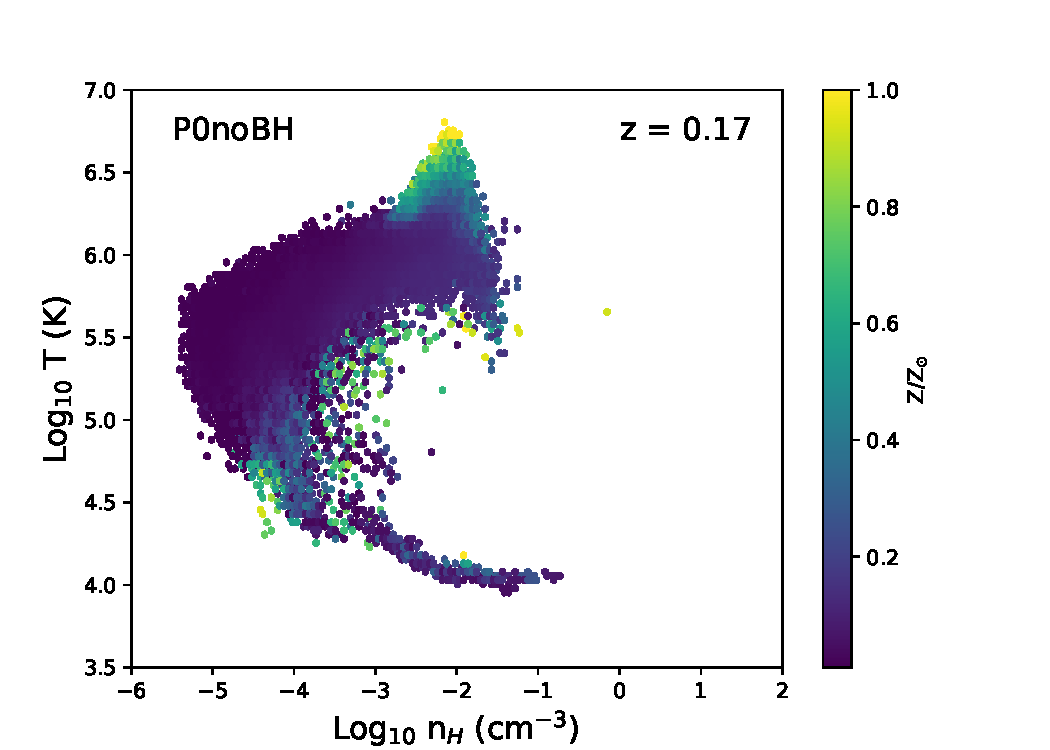
\includegraphics[angle=0]{P0noBH_phasediagram_metallicity}}
\resizebox{0.35\hsize}{!}{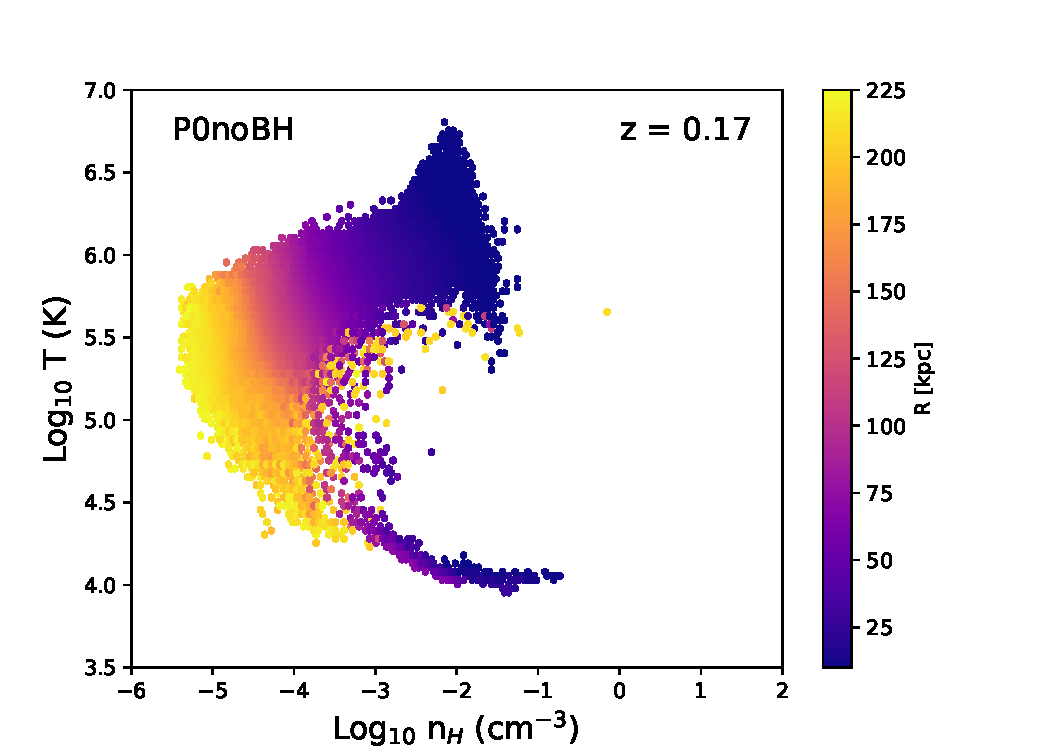
\includegraphics[angle=0]{P0noBH_phasediagram_Rkpc}}}

\centerline{\resizebox{0.35\hsize}{!}{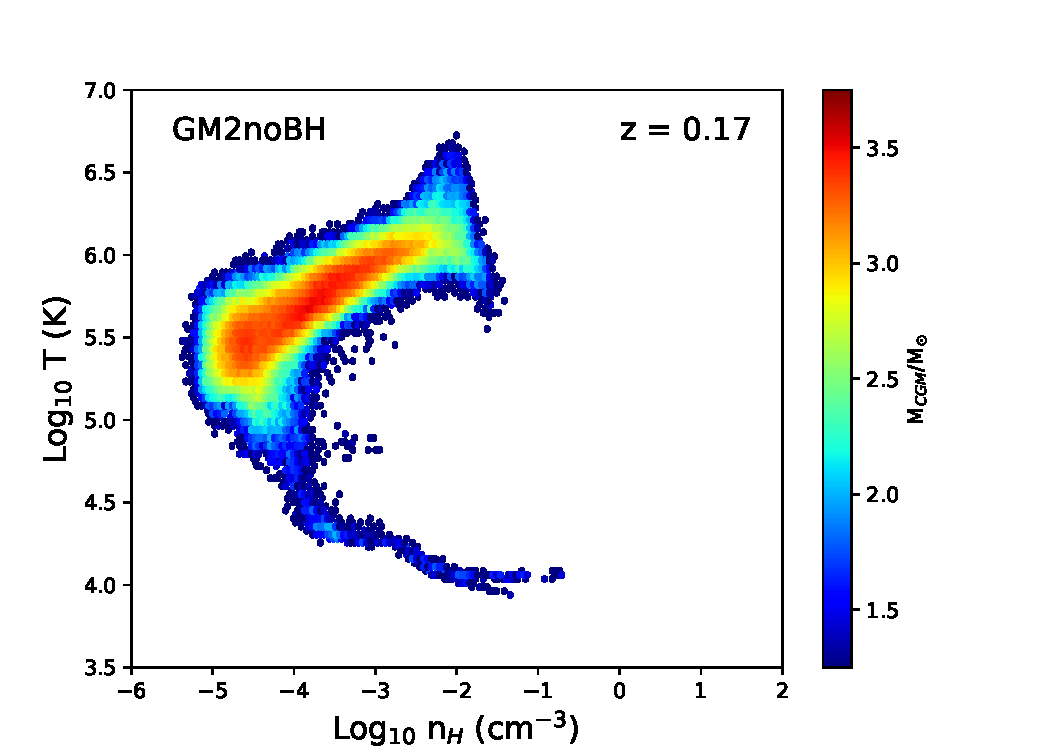
\includegraphics[angle=0]{GM2noBH_phasediagram_mass}}
\resizebox{0.35\hsize}{!}{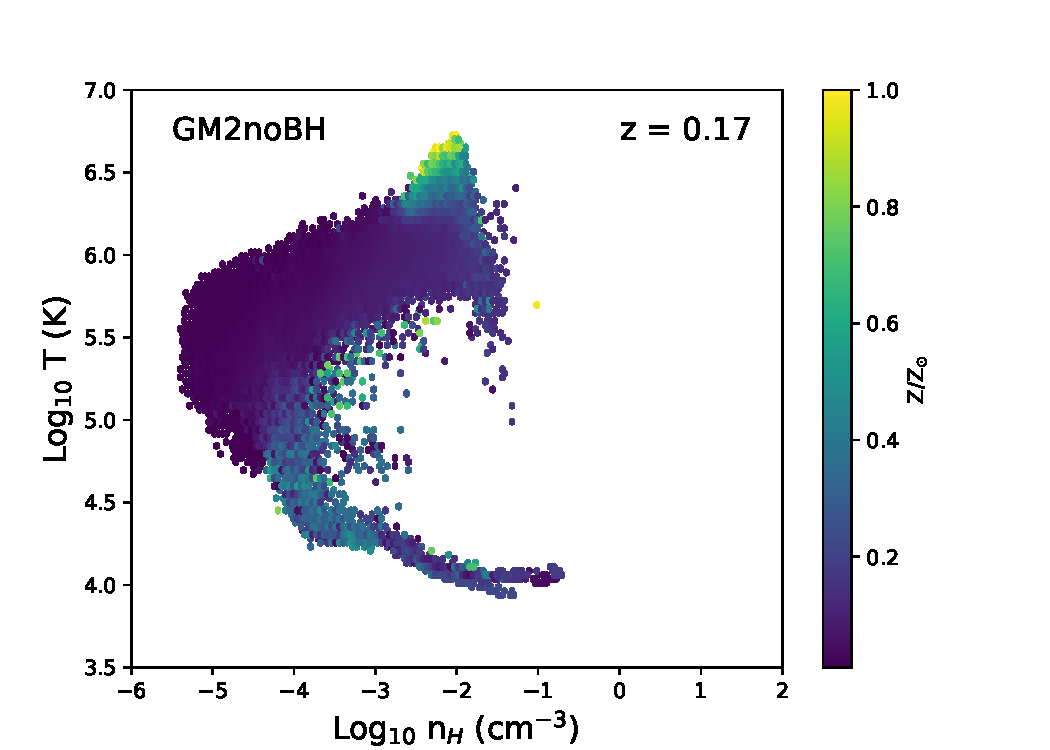
\includegraphics[angle=0]{GM2noBH_phasediagram_metallicity}}
\resizebox{0.35\hsize}{!}{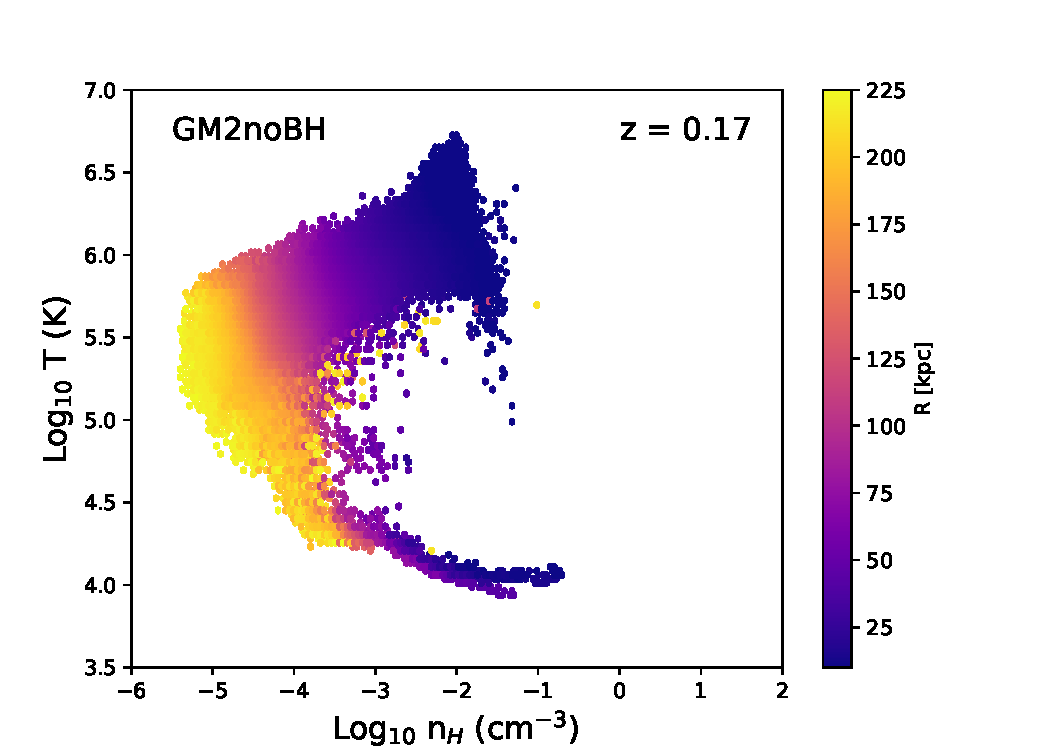
\includegraphics[angle=0]{GM2noBH_phasediagram_Rkpc}}}

\caption[]{Phase diagrams of the temperature and density of the star forming zoom-in galaxy, P0 (\textit{Top row} with BH physics, \textit{Middle row} without), and the quenched galaxy, GM2 (\textit{Bottom row}). \textit{Left:} As we noted, the phase diagrams of galaxies with BH hole physics show stark differences between the star forming (P0 and GM1) and quenched cases (GM2 and GM3).  particularly in the highest temperature and density gas. \textit{Middle:} The same phase diagram showing temperature and density, however, the colorbar is weighted by the average metallicity of the star in each bin. We note that the high density, high temperature gas we see in the star forming P0, is also the highest metallicity gas in the CGM. \textit{Right:} Similarly, a phase diagram with the colorbar now weighted by the average distance from the center of the galaxy of the gas particles in each bin. The concentration of gas at high density and temperature \textit{and} high metallicity also appears to be the gas closest to the center of the galaxy. However, this gas is also not present in the noBH physics case. We conclude that due to the active star formation in P0 in tandem with the AGN physics at play, this excess of gas comes from gas that has been ejected from the disk due to AGN feedback. Therefore explaining it's significant absence from the phase diagrams of P0 without BH physics and GM2.}
\label{figure:phasediagrams_z_R}
\end{figure*}


\subsection{Qualitative CGM Properties}

% We identify halos using AHF and result in halos of this mass range.
Individual halos in the ROMULUS25 cosmological volume and in the individual zoom-in galaxies are extracted using the Amiga Halo Finder (AHF) \citep{Knollmann2009} and central SMBH positions and velocities are defined relative to the center position and inner 1 kpc center-of-mass velocity of their host halo, respectively. From R25, we specifically examine Milky Way-mass halos which are defined as halos between 5 $\times$ $10^{11}$ and 2 $\times$ $10^{12}$ M$_{\odot}$ and are at least twice a virial radii from their nearest neighbor (to exclude any satellites). All zoom-in galaxies are isolated with a minor merger at z $\sim$ 1.  

% We define the CGM on this scale and in this environment for our galaxies.
The CGM of each individual galaxy halo (within the R25 galaxies and our zoom-ins) is defined as the mass enclosed in an annulus from 10 kpc from the center position out to a virial radius defined as the radius at which 200 times the critical density, $\rho_c$, where $\rho/\rho_c$ = 200. Figure \ref{phasediagrams} shows the phase diagrams of the CGMs of the 4 zoom-in galaxies with and without BH physics. Examining the CGM phase diagrams for the GMs that \text{include} BH physics (\textit{Left Column}), we note the following key differences: less overall mass from the uppermost (P0) to lowermost (GM3) figure; variations in the amount of cool, dense gas (T \textless 10$^{4.5}$, n$_H$ \textgreater 10$^{-3}$); and the lack of hot, dense gas (T \textgreater 10$^{5.5}$, n$_H$ \textgreater 10$^{-3}$) in the phase diagrams of GM2 and GM3, our quenched galaxies. Similarly, examining the CGM phase diagrams that \textit{exclude} BH physics (\textit{Right Column}), we don't see any significant differences. 

The first of the differences between CGM phase diagrams with BH physics is unsurprising, as it correlates directly with the final halo mass of the galaxies. P0 results in the most massive halo at z $\sim$ 0, while GM3 results in the least massive (Table \ref{table:BHdata}). The second of these differences \textbf{[FINISH ANALYSIS ON COOL DENSE TAIL]}.

We are most interested in the last difference: the lack of the hot, dense gas in the quenched galaxies that is present in the star forming galaxies, P0 and GM1. We note that this feature is also present in the CGM diagrams of the galaxies \textit{without} BH physics, which all result in star forming, disked galaxies. Figure \ref{figure:phasediagrams_z_R} further examines this difference with the same CGM phase diagrams of P0 and GM2 colored by mass, metallicity, and distance from the center of the galaxy, with (\textit{Two Upper Rows}) and without (\textit{Two Lower Rows}) BH physics. The hot, dense gas in P0 with BH physics (\textit{Upper Row}) appears to be mostly comprised of high metallicity gas that is close to the disk (R \textless 50 kpc). Further examining this gas, we find that 3 $\%$ of the CGM gas has metallicity Z \textgreater Z$_{\odot}$ at z = 0.17. Furthermore, of this 3 $\%$, 23 $\%$ is between 10 and 20 kpc from the center of the galaxies. For GM1, the CGM is comprised of 7.6 $\%$ gas with Z \textgreater Z$_{\odot}$ with nearly 50 $\%$ of that gas between 10 and 20 kpc. Contrastingly, a negligible amount of the CGM of both GM2 and GM3 have Z \textgreater Z$_{\odot}$ at z = 0.17. The CGMs of the four galaxies without BH physics also have small amounts of gas with Z \textgreater Z$_{\odot}$, from 0.1 $\%$ in P0noBH to 0.04 $\%$ in GM3noBH. These percentages of high metallicity gases in P0 and GM1 with BH physics point to metal exchange in the galaxy that is strongly dependent on the SMBH (which we discuss further in Section \ref{Result:metalsbyBH}). It's interesting to note that the removal of the BH physics in all four zoom-ins makes little difference in the final gas phase properties of the main halo (Table \ref{table:noBHdata}). Nevertheless, the differences we see in the CGMs of these galaxies, both with and without BH physics, don't seem to have a significant effect on the OVI that we see in the galaxies, as we explore below.

\begin{figure*}[ht!]
\centerline{\resizebox{0.48\hsize}{!}{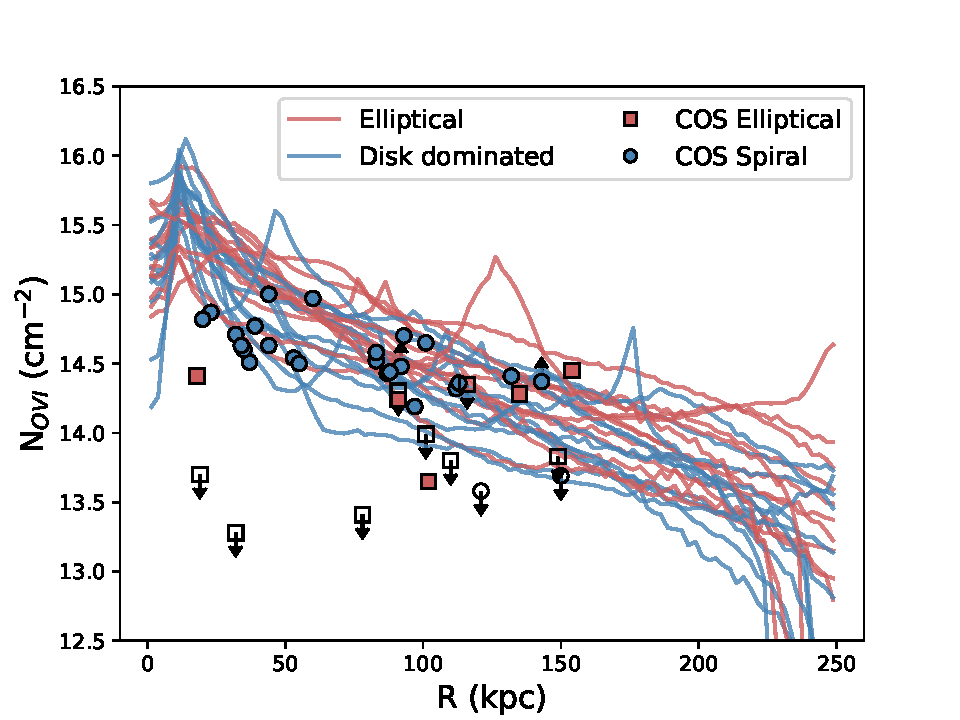
\includegraphics[angle=0]{Novi_profile_ALLMWROM_plusobs}}
\resizebox{0.48\hsize}{!}{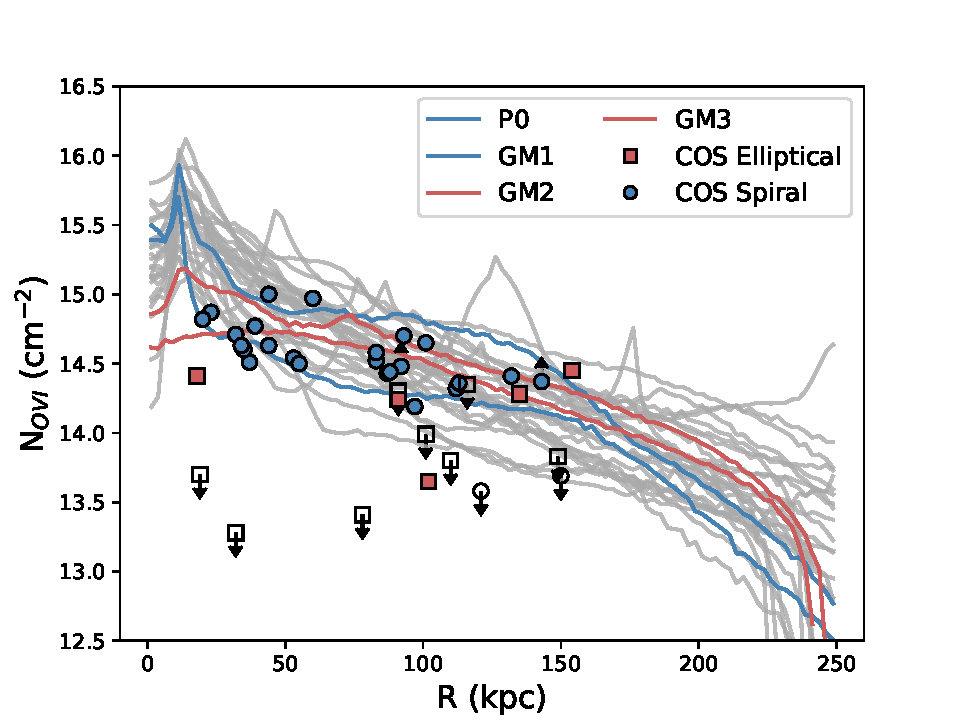
\includegraphics[angle=0]{Novi_profile_ALLMWROM_GMs_plusobs}}}
\caption[]{\textit{Left:} Mean column densities of OVI as a function of radius for all Milky Way mass halos in the R25 simulation. Blue and red lines distinguish between disk dominated spirals and quenched elliptical galaxies within the R25 simulation. \textit{Right:} Column densities of OVI in our 4 zoom-in galaxies. Grey lines indicate R25 MW galaxy column densities from \textit{Left}. Blue solid lines describe our two star forming galaxies, P0 and GM1. GM4-7, our passive galaxies, are in solid red. Filled circles and squares indicate spirals and ellipticals from the COS-Halo Survey dataset. Unfilled squares indicate upper limits.}
\label{figure:ROM_Novi_vs_b}
\end{figure*}

\subsection{OVI as a Tracer for Virial Temperature}
\label{Result:OVIasTtracer}
% We calculate the column densities of OVI like this.
Column densities of OVI are calculated using the analysis software Pynbody (Pontzen 2013). Oxygen abundances is traced throughout the integration of the simulation and  ionization states are calculated during post-processing, assuming optically thin conditions and a \cite{Haardt2012} ultraviolet radiation field at z = 0. Recent papers \textbf{[CITE]} have raised concerns that this UV background is too strong \textbf{[CITE]}; however, since our primary concern is the abundance of OVI which is considered to be collisionally ionized rather than photoionized \textbf{[CITE]}, our choice of UV background should not affect our results. We use the CLOUDY software package \citep{Ferland1998,Stinson2012} to create models with varying temperature, density, and redshift to determine OVI fractions for all the gas in each simulated galaxy. Figure \ref{figure:ROM_Novi_vs_b} shows the column densities of OVI as a function of radius \textbf{(Need to change this to impact parameter; Current profiles are created when galaxies are in a face-on orientation.)} for our 25 R25 MW-mass galaxies. Red and blue lines describe quenched and star forming galaxies within the sample, respectively. The COS-Halo Survey dataset is plotted on top in black, with squares and circles distinguishing between elliptical and spiral galaxies. Upper and lower limits are designated with arrows and unfilled markers. The R25 galaxies well match the observations from the COS-Halo Survey; however, we note that they are systematically higher than the upper limits of the more massive ellipticals in the survey. (See \ref{Discuss}) We further compare the column densities of OVI in the R25 galaxies to the 4 zoom-in galaxies with BH physics and find that these galaxies also well match the observed column densities of COS-Halo and fall within the range of the R25 galaxies (Figure \ref{figure:ROM_Novi_vs_b}b). 

Figures \ref{figure:ROM_Novi_vs_b} and \ref{GMandNOBH_Novi_vs_b} make it clear that our simulations reproduce the column densities of OVI in the CGM; however, this conclusion is not the only important feature of these plots. In addition, we note that \textit{the column densities of OVI in the CGMs of these galaxies does not seem to depend on the assembly history of the galaxy.} We see this in both R25, which in addition to providing evidence for this initial result also gives cosmological credence to our suite of GM galaxies, and our four GM galaxies that include BH physics. We confirm our result with Patient 0 and its GMs, which include two star forming galaxies and two quenched galaxies, all of which well match the observations of COS-Halo despite differing formation histories. (Figure \ref{GMandNOBH_Novi_vs_b})


\begin{figure}[h!]
\centerline{\resizebox{0.98\hsize}{!}{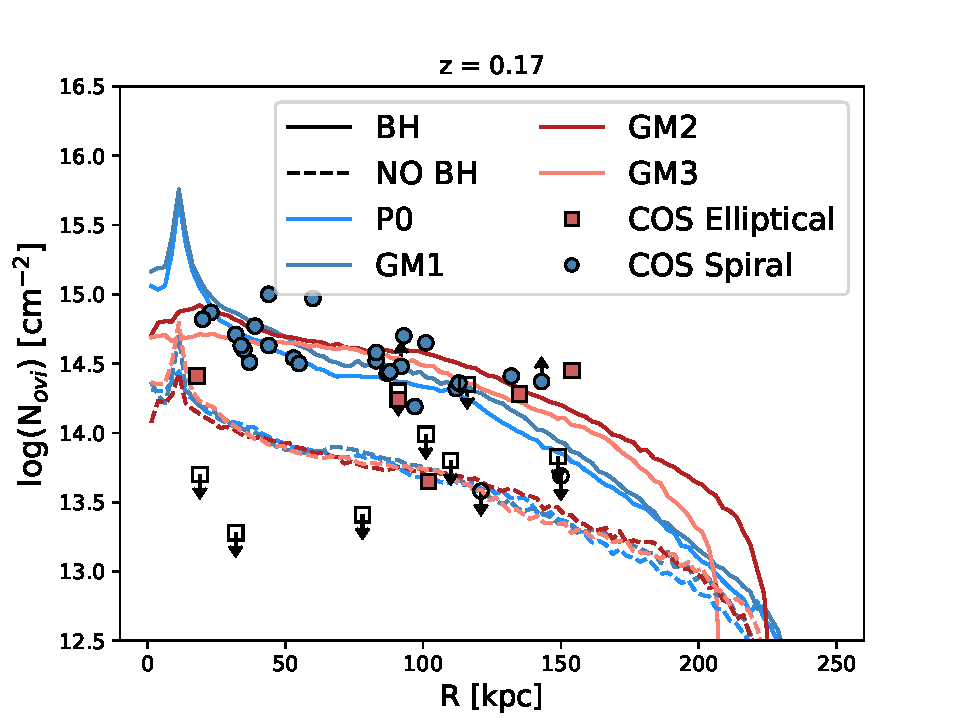
\includegraphics[angle=0]{ALLGMs_plusnoBH_Novi_R}}}
\caption[]{Column density profiles of OVI in our 4 zoom-in galaxies with (solid lines) and without (dashed lines) BH physics. P0 and GM1, our two star forming galaxies are colored as light blue and dark blue, respectively. Our quenched galaxies, GM2 and GM3, are labeled in dark red and pink, respectively.}
\label{GMandNOBH_Novi_vs_b}
\end{figure}

\begin{figure}[ht!]
\centerline{\resizebox{1.\hsize}{!}{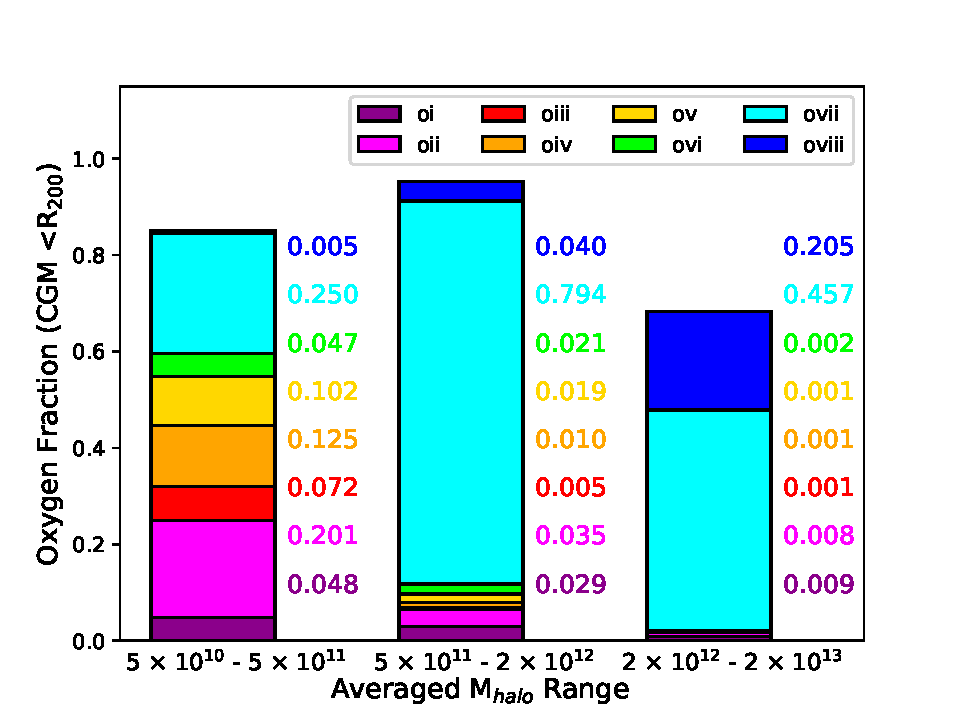
\includegraphics[angle=0]{OPPEN_fig10_ROMgxys_averaged}}}
\caption[]{Oxygen ion fractions in the CGM of our 25 MW-mass galaxies and 11 high mass galaxies from R25. Log M$_{Halo}$ for each halo are labeled in white text. [\textbf{Under construction}]}
\label{oppenheimer}
\end{figure}

Figure \ref{oppenheimer} shows the average fractions for all the ions of oxygen within three mass ranges: low mass (5 $\times$ 10$^{10}$ \textemdash 5 $\times$ 10$^{11}$ M$_{\odot}$), Milky Way-mass (5 $\times$ 10$^{11}$ \textemdash 2 $\times$ 10$^{12}$ M$_{\odot}$), and high mass (2 $\times$ 10$^{12}$ \textemdash 2 $\times$ 10$^{13}$ M$_{\odot}$). The OVI fractions decrease from the MW-mass range to the high mass regime due to the increase in virial temperature which moves from a value close to the ionization peak for OVI, $\sim$ 10$^{5.5} K$) to 10$^{6.3}$ K. From this study, we determine that morphological evolution of the galaxy doesn't correlate with the evolution of the CGM, as described by the column densities of OVI. Instead, it appears that the mass of the galaxy, and connectedly its virial temperature [Table \ref{table:BHdata}], plays a more significant role in determining the amount of OVI seen in the CGM.


\subsection{Metal Transport by the SMBH}
\label{Result:metalsbyBH}

We examine the column densities of OVI in the CGMs of our 4 zoom-in galaxies \textit{without} BH physics and compare them to the cases where BH physics is included. Figure \ref{GMandNOBH_Novi_vs_b} shows the column densities of OVI in the CGM of all four of our zoom-in galaxies with BH physics (solid lines) and without (dashed lines). We can see that in the cases where BH physics is not included, the values of N$_{OVI}$ are significantly lower implying that the presence of the AGN must play an important role in populating OVI in the CGM. We look to the temperature, mass, density, and metallicity of the CGM to investigate the cause of this decrease in OVI. (Figure \ref{T_M_rho_Z})

The difference between the CGMs of these two cases appears to come directly from the change in metallicity due to the lack of black hole activity. (Figure \ref{T_M_rho_Z}) We examine the metallicity of the disk to look for further clues about how the lack of AGN activity is affecting the galaxy. Figure \ref{DISK_Z} shows that, in the galaxies without BH physics, the metals produced in the disk aren't driven into the CGM due to the lack of AGN feedback. This result is also consistent with what we see in Figure \ref{figure:phasediagrams_z_R}. The lack of high metallicity (Z \textgreater Z$_{\odot}$) in the CGM phase diagrams of the galaxies with no BH physics (\textit{Right Column}) confirms the fact that metals are not being driven out of the disk. Surprisingly, however, the feedback doesn't seem to play a role in significantly heating or excavating the CGM gas, but it appears the the AGN's feedback is pivotal in \textit{transporting the metals} from the center of the galaxy out into the CGM. \textit{The AGN plays a significant role in physically driving the metals out of the disk and into the outer regions of the CGM.}

\textbf{[Include discussion about metal flux into and out of galaxy (once complete); comparisons between observations and amount of total metals in disk (plus metal gradients)]} 


\begin{figure*}
\centerline{\resizebox{0.45\hsize}{!}{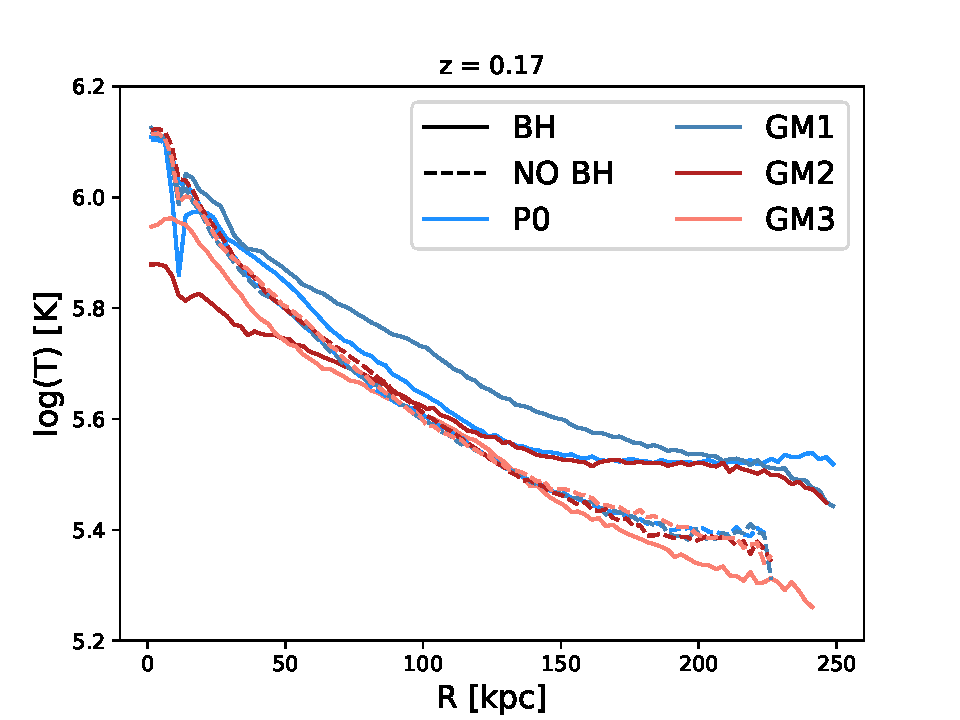
\includegraphics[angle=0]{ALLGMs_plusnoBH_T_R}}
\resizebox{0.45\hsize}{!}{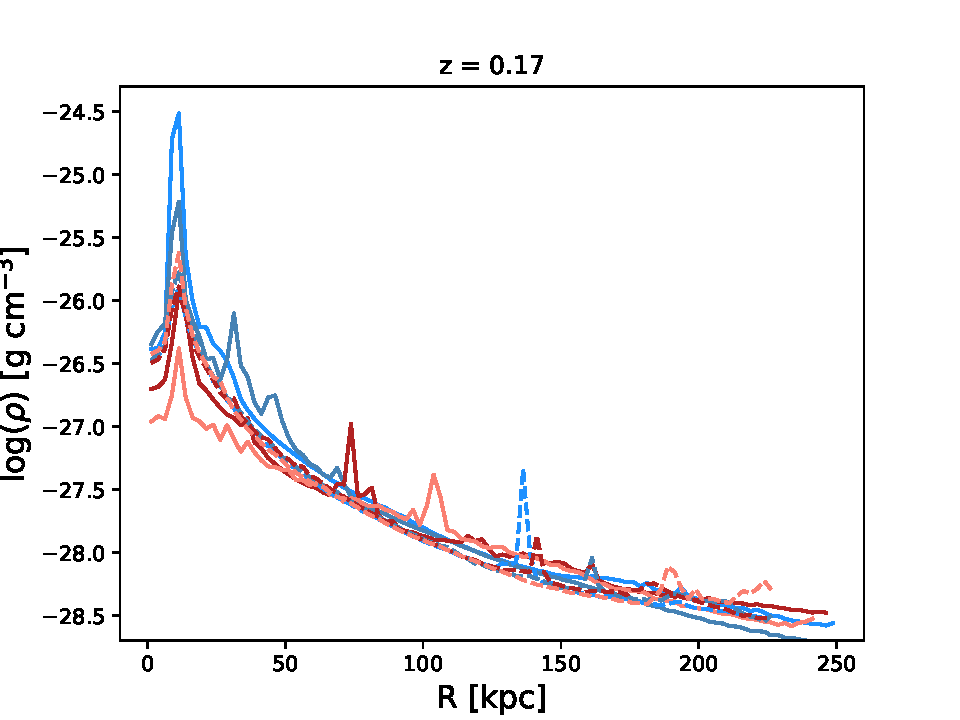
\includegraphics[angle=0]{ALLGMs_plusnoBH_rho_R}}}
\centerline{\resizebox{0.45\hsize}{!}{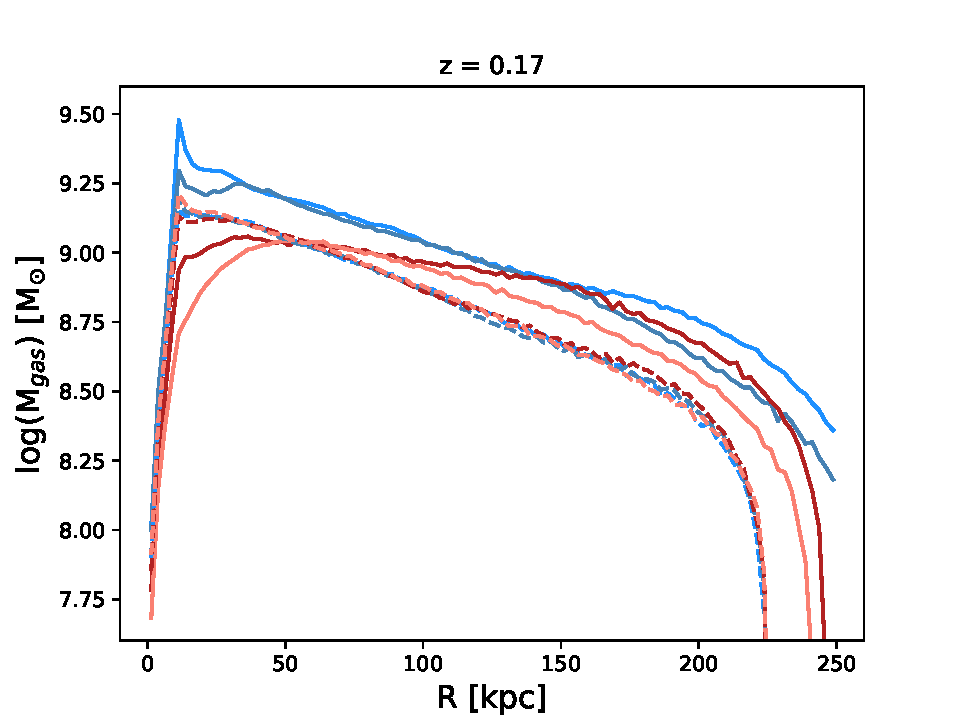
\includegraphics[angle=0]{ALLGMs_plusnoBH_totgasmass_R}}
\resizebox{0.45\hsize}{!}{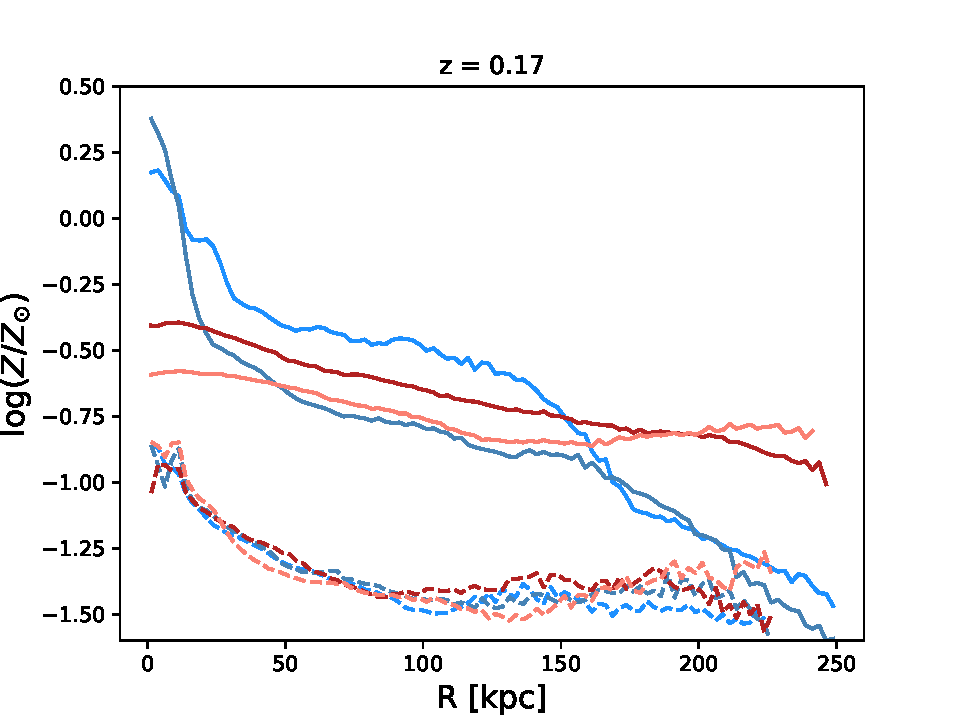
\includegraphics[angle=0]{ALLGMs_plusnoBH_Z_R}}}
\caption[]{Temperature, Total Mass, Total Density, and Metallicity profiles of the CGM of our 4 zoom-in galaxies with and without BH physics. Colors and linestyles as in Figure \ref{GMandNOBH_Novi_vs_b}.}
\label{T_M_rho_Z}
\end{figure*}

\begin{figure}[h!]
\centerline{\resizebox{1.05\hsize}{!}{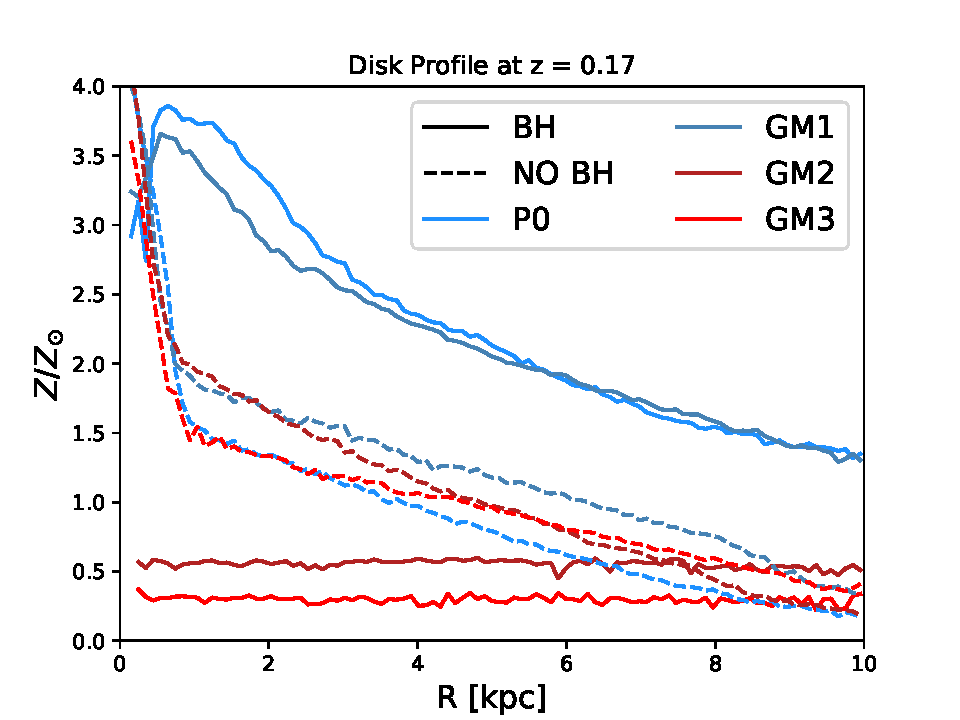
\includegraphics[angle=0]{ALLGMs_DISKmetals_R_plusnoBHs}}}
\caption[]{Metallicity profile of the gas within the disk of our 4 zoom-in galaxies with and without BH physics. Colors and line styles as in Figure \ref{T_M_rho_Z}. Without the black hole physics, metals remain trapped near the center of the disk with no mechanism to propagate out into the CGM.}
\label{DISK_Z}
\end{figure}


% ########## END OF RESULTS ###########
% #####################################

% #####################################
% ########### DISCUSSION ##############
% #####################################
\section{Discussion} 
\label{Discuss}

Questions to expound on:
Limitations of the simulations
Comparisons with other groups: Oppenheimer, Suresh, Hummels(Fire)?
What questions remain/are raised by results 


% ########## END OF DISCUSSION ###########
% ########################################


% #####################################
% ########### CONCLUSION ##############
% #####################################

\section{Conclusion} 
\label{Conclude}

\textbf{Result 1: OVI as a Tracer for Virial Temperature of the Halo}

The combined, consistent results of the cosmological R25 and our 4 zoom-in galaxies (which include BH physics) imply a mechanism by which column densities of OVI are set by the virial temperature of the CGMs host galaxy. They aren't affected by the evolution of a disk. Their phase diagrams also lack significant difference in their overall assembly history, except where more gas is clearly present in the higher mass galaxies. Therefore, we surmise that the differences in the CGM are not determined by whether or not a galaxy quenches but rather these conditions for OVI are primarily set by the virial temperature of the galaxy. 

These results are consistent with those of Oppenheimer et. al. 2016 who used a suite of EAGLE simulated galaxies to examine the bimodality of OVI column densities (further discussed in [Tumlinson 2011]) in star forming and quenched galaxies. They argue that the star forming galaxies (10$^{11}$ - 10$^{12}$), which were found to have a higher fraction of OVI, were at the right virial temperature to maximize OVI production, while their quenched galaxies (10$^{12}$ - 10$^{13}$) had high enough virial temperatures such that the dominant ionization state was not OVI but rather OVII or above. Oppenheimer et. al. 2016 argues that the OVI content was not a tracer of star formation directly, but rather a more direct thermometer for the temperature of the halo.

We note that the quenched galaxies in our sample are smaller in mass than our star forming galaxies, unlike those in Oppenheimer, explaining the lack of bimodality that we observe. While all the GMs are in the mass range to have virial temperatures which optimize OVI, we further examine the R25 simulation's higher mass, passive galaxies in addition to the MW-mass galaxies (which have virial temperatures spanning 5.8 $\times$ 10$^{5}$ K $\textemdash$ 1.1 $\times$ 10$^{6}$ K) to see if the bimodality appears. (Figure \ref{oppenheimer}) We determine that the OVI still provides a direct thermometer for the temperature of the halo. [\textbf{Under construction}]

Furthermore, examining galaxies with masses larger than our MW-mass GMs (\textgreater 2 $\times$ 10$^{12}$) from the R25 suite, we see that the column densities of OVI decrease as the ionization peak of OVI is surpassed by these halos. Since the virial temperature is higher, the oxygen is likely to be ionized to a higher ionizations state (OVII or OVII), which we show is the case in Figure \ref{oppenheimer}. [\textbf{Under construction}]

\textbf{Result 2: AGN as driver for metals in the CGM}

Our result that the AGN acts a physical driver for metals in the CGM has interesting consequences. Previous studies have examined the effect of heating on the CGM as the AGNs energy input may put the gas into phases which optimize the production of OVI. \citep{Suresh2017} Others have proposed that the feedback from AGN may physically drive outflows of gas out of the galaxy, resulting in a lower density CGM and therefore lower densities of OVI. Neither of these cases are what we see. \textit{Instead, we see a suite of CGM which rely on the AGN for the propagation of metal mass (but not total gas mass) into the outer galaxy and OVI columns which depend on the virial temperature of the galaxy.} (Figure \ref{DISK_Z})

% ####### END OF CONCLUSIONS ##########
% #####################################

\acknowledgments
Acknowledgements

\bibliography{/Users/the_neekster/Documents/MENDELEY/MEND_bibtexfiles/SanchezCGM2018.bib}
% ADD THIS LATER TO BIB
% @misc{pynbody,
%   author = {{Pontzen}, A. and {Ro{\v s}kar}, R. and {Stinson}, G.~S. and {Woods},
%      R. and {Reed}, D.~M. and {Coles}, J. and {Quinn}, T.~R.},
%   title = "{pynbody: Astrophysics Simulation Analysis for Python}",
%   note = {Astrophysics Source Code Library, ascl:1305.002},
%   year = 2013
% }

\end{document}

